\section{静電気力・電場・電位}

% ===========================================================================
%  再編（2026-09-23）：第4章 電磁気学 の第24回（電磁気の初回）．
%  原本の 第29回「クーロンの法則・電場」の全体（29.1〜29.4）と，
%  第30回「電位・電位によるエネルギー」の全体（30.1・30.2）を1回に統合した．
%    `saihen/電磁気_例題配分.md`「第24回 静電気力・電場・電位」の通り．
%
%  ・練習は13題．旧㉙[1]〜[7]・旧㉚[8]〜[11][13][14] と，練習へ降ろした原本例題4を収録し，
%    A問題の㉙[1]と㉚[8]を1題に統合した（設問は1つも失われていない）．
%      ［34］＝㉙[1]＋㉚[8]（A問題の統合。クーロン力／点電荷の電場／電位差の基本）
%      ［35］＝㉙[2]（クーロンの法則）      ［36］＝㉙[3]（力のつり合い）
%      ［37］＝㉙[4]（クーロン力と電場）    ［38］＝㉙[5]（電気力線の作図）
%      ［39］＝原本例題4（箔検電器）        ［40］＝㉙[6]（静電誘導の4段階）
%      ［41］＝㉚[9]（静電気力のする仕事）  ［42］＝㉚[10]（一様電場と電位差）
%      ［43］＝㉚[11]（点電荷による電場と電位）
%      C問題 ［44］＝㉙[7]（立方体）／［45］＝㉚[13]（等電位線と仕事）／
%            ［46］＝㉚[14]（電場と仕事）
%    ［39］（原本例題4）を［40］（旧[6]）の直前に置いたのは，例題4が静電誘導の
%    「定性的な説明」，旧[6]が「各操作の図示」で，前者が後者の導入になるため
%    （`saihen/電磁気_例題配分.md`「練習へ移す3題の扱い」）．
%    旧㉚[12]（無限遠へ飛び去る初速）は電位による位置エネルギーの応用なので
%    第29回（電場・磁場中の荷電粒子の運動）へ送った．
%
%  ・例題は5題．原本の 例題1・2・3・5・6 をそのまま採用した．
%    電磁気（原本 第4章）の例題は章の先頭から1・2・3…と数えるので，
%    この回が【例題1】〜【例題5】になる（\setcounter{nombre}{0}）．
%    原本例題4〈箔検電器〉は練習［39］へ，原本例題7〈電位による位置エネルギー〉は
%    第29回へ送った．
%
%  ・原本の誤り・不統一を直した（いずれもコメントで明記）：
%      (a) 旧 physics_ch29.tex 29.4 の「同種の殿下同士は」→「同種の電荷同士は」（変換ミス）．
%      (b) 旧 physics_ch29.tex 29.1 の「$q_2$[Cの物体が」→「$q_2\U{C}$の物体が」（括弧の脱落）．
%      (c) 練習［34］(5)（旧㉚[8](2)）の解答の $V=k\dfrac{q}{Q}$ → $V=k\dfrac{q}{r}$．
%          原本の解答の式だけが誤りで，代入した数値（$2.0$）は距離である．
%      (d) 旧 physics_ch30.tex 30.1 の点電荷の電位のまとめで
%          $V(x)=k\dfrac{Q}{r}$ と左辺だけ $x$ の関数のまま残っていたのを $V=k\dfrac{Q}{r}$ に．
%      (e) 単位を $[\mathrm{N}]$ 等の直書きから \U{} に，強調を {\bf } から {\gtfamily } に，
%          点の名前を \mathrm{} に統一した（第21〜23回に合わせた）．
%
%  ・原本の本文に無く，練習・例題が前提にしていたものを加筆した：
%      ・24.3 に「電気力線は電場の強い所ほど密」だけでなく，
%        「正電荷から出る本数は電気量だけで決まる」ことを明示（例題3・練習［38］が使う）．
%      ・24.5 に等電位面（等電位線）の定義と「電場は等電位面に直交する」を追加．
%        原本は例題5の指針で初出だったが，例題5(2)・練習［45］［46］がこれを使う．
%      ・24.6 に「電位はスカラーなので向きを考えず単純和でよい」を明示
%        （練習［43］［45］［46］の要）．
%
%  ・図：講義編の図（text2_p26/28/29/30/31/32/35_fig*）はそのまま流用し，
%    網点の濃い4枚だけ fig/ に明るくした別名を作った（原本は書き換えない）．
%    例題・練習・解答の図は texify_draft/mkfig_new24.py で切り出せる．
%    例題の解答の作図（例題3・例題4）は原本に無いので TikZ で自作した
%    （texify_draft/mkfig_new24ans.py）．
%  ・wrapfigure は使わず zuright / center だけで組んだ（組版チェックリスト §3.8）．
% ===========================================================================

% 例題番号：電磁気（原本 第4章）の例題は章の先頭から1・2・3…
\setcounter{nombre}{0}

\subsection{クーロンの法則}

物体は種々の原子が組み合わさって作られているが，その原子は正の電気量を持つ原子核と，負の電気量を持つ電子から構成されており，原子核は正の電気量を持つ陽子と電気量を持たない中性子とからできている．
この陽子と電子の電気量の絶対値は等しく，この値を{\gtfamily 電気素量}$e$で表す．
電気量は{\gtfamily クーロン}$\U{C}$を単位として用いる．
この単位を用いると，電気素量は$e\fallingdotseq 1.60\times 10^{-19}\U{C}$である．

通常の物体は陽子の数と電子の数が等しいため，正負の電気量が打ち消しあって電気的に中性の状態になっているが，電子は原子核に比べて圧倒的に軽いため，物質によっては容易に引き抜いたり，逆に付け加えたりすることができる．
そのため，物体に余分に電子を与えると物体は負に帯電し，逆に物体から電子を取り去ると物体は正に帯電する．
すなわち，\,\AnaB{電子の過不足}\,により物体は帯電する．
帯電体の持つ電気を{\gtfamily 電荷}という．

\begin{zuright}{56mm}
\hspace{1zw}一般に，電荷を持った物体同士は互いに力を及ぼしあうことが知られている．
電気量の大きさが$q_1\U{C}$，$q_2\U{C}$の物体が距離$r\U{m}$だけ隔てて置かれているとき，2つの電荷が{\gtfamily 同符号の場合は斥力}を，{\gtfamily 異符号の場合は引力}を及ぼしあう．
力の向きは，いずれも{\gtfamily 2つの電荷を結ぶ直線の方向}である．
一方が他方に及ぼす力と，他方が一方に及ぼす力とは，作用・反作用の関係にあって大きさが等しく向きが逆である．
\zusep
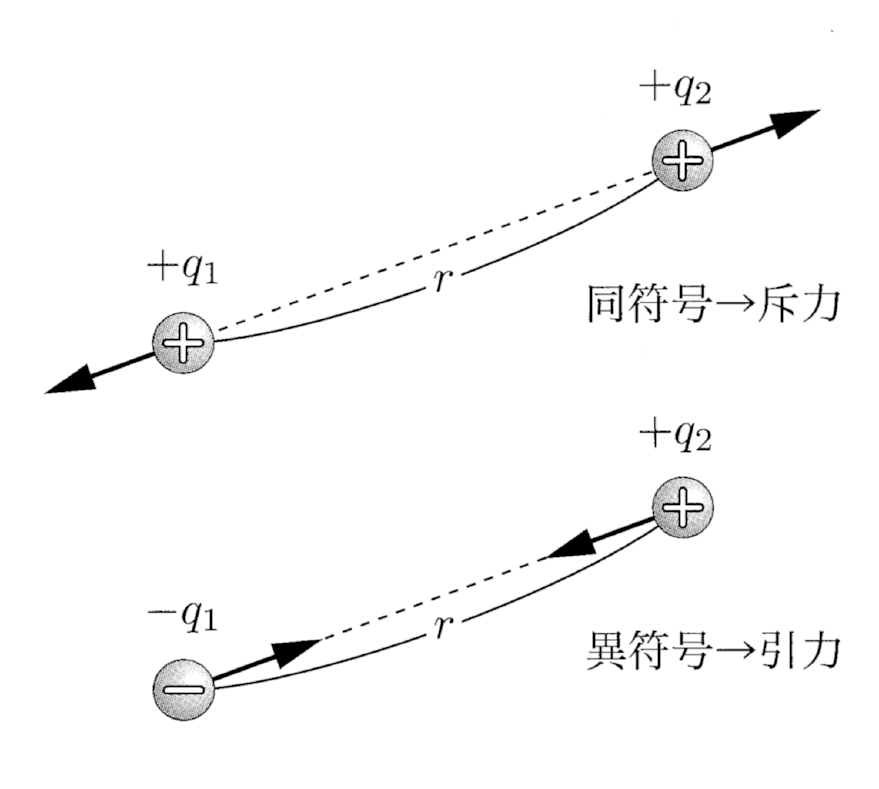
\includegraphics[keepaspectratio,width=56mm]{fig/n24_zu_coulomb.png}
\end{zuright}

\noindent その大きさ$f\U{N}$は，
\AnaBD{f=k\frac{|q_1q_2|}{r^2}\U{N}}
で表される．
この力のことを{\gtfamily クーロン力}（静電気力）と呼ぶ．
比例定数$k\U{N\cdot m^2/C^2}$をクーロンの法則の比例定数といい，真空中での値は$k\fallingdotseq 8.9876\times 10^9\U{N\cdot m^2/C^2}$である．

\begin{matome}{クーロンの法則}
 \hspace{3mm} 電荷は互いに力を及ぼしあう．電荷の符号が{\gtfamily 同符号なら斥力，異符号なら引力}\\[1mm]
 \hspace{8mm} 向きは2つの電荷を結ぶ直線の方向，大きさは\hspace{3mm}$f=k\dfrac{|q_1q_2|}{r^2}\U{N}$\\[1mm]
 \hspace{3mm} {\gtfamily 電気量には絶対値をつけて代入し，向きは符号から別に決める}
\end{matome}

クーロンの法則の比例定数は，後で述べる真空の誘電率$\varepsilon_0\U{C^2/N\cdot m^2}$と
\[k=\frac{1}{4\pi\varepsilon_0}\]
の関係がある．$\varepsilon_0\fallingdotseq 8.854\times 10^{-12}\U{C^2/N\cdot m^2}$である．

%%%%%%%%%%  例題1（24.1 の直後。原本の【例題1】）  %%%%%%%%%%%%%%%%%%%%
\bsNeed{86mm}
\begin{reidaiunit}
\begin{reidai}{クーロンの法則}
\begin{zuright}{52mm}
\hspace{1zw}図のように，原点からそれぞれ距離$d\U{m}$の点$\mathrm{A}$，$\mathrm{B}$に同一の電気量$+q\U{C}$を持つ正の点電荷を固定し，さらに位置$(0,\ d)\U{m}$の点$\mathrm{C}$に$-q\U{C}$の負の点電荷を配置した．クーロンの法則の比例定数を$k\U{N\cdot m^2/C^2}$として以下の問に答えよ．
\zusep
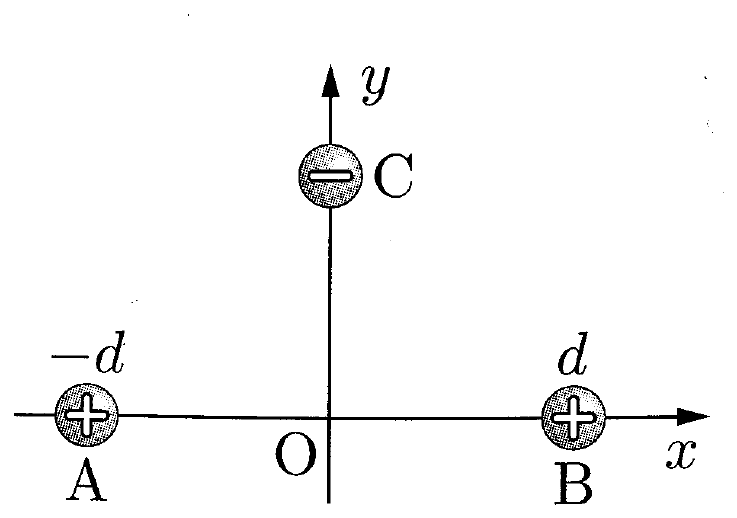
\includegraphics[keepaspectratio,width=52mm]{fig/n24_ex1_zu.png}
\end{zuright}
\begin{komon}
\ko{1} 点$\mathrm{A}$の電荷が点$\mathrm{C}$の電荷に及ぼすクーロン力の大きさおよび向きを答えよ．
\ko{2} 点$\mathrm{C}$の電荷が受けるクーロン力の大きさおよび向きを答えよ．
\ko{3} さらに電気量$+q\U{C}$の正電荷を$y$軸上に置くことにより，点$\mathrm{C}$の電荷が受けるクーロン力の合力を$0\U{N}$にしたい．正電荷を配置するべき位置を求めよ．
\end{komon}
\end{reidai}

\begin{sisinE}
クーロン力を考える場合は，{\gtfamily 向きと大きさを分けて}考える．まず電気量の絶対値を$f=k\dfrac{|q_1q_2|}{r^2}$に代入して大きさを求め，つぎに同符号か異符号かを見て向きを決め，図中に矢印で記入していく．

2つ以上の電荷から力を受けるときは，力はベクトルであるから{\gtfamily 大きさの単純和ではなくベクトル和}を取る．本問では$\mathrm{A}$と$\mathrm{B}$が$y$軸について対称なので，$x$成分が打ち消し合うことが図から読み取れる．
\end{sisinE}

\Key{電荷の符号が同符号なら斥力，異符号なら引力，2点を結ぶ直線方向で作用\quad $f=k\dfrac{|q_1q_2|}{r^2}\U{N}$}

\begin{kaitou}
\begin{komon}
\ko{1} $\overline{\mathrm{AC}}=\sqrt{d^2+d^2}=\sqrt{2}\,d\U{m}$であるから，その大きさは
       \[f=k\frac{|(+q)\cdot(-q)|}{\left(\sqrt{2}\,d\right)^2}=\frac{kq^2}{2d^2}\U{N}\Ans\]
       また$\mathrm{A}$の電荷と$\mathrm{C}$の電荷は異符号であるから引力であり，向きは
       \[\overrightarrow{\mathrm{CA}}\text{の向き}\Ans\]
\ko{2} 点$\mathrm{B}$の電荷が$\mathrm{C}$に及ぼす力も同じ大きさ$\dfrac{kq^2}{2d^2}\U{N}$の引力で，向きは$\overrightarrow{\mathrm{CB}}$である．この2力のベクトル和を取ると，$x$成分は打ち消し合い，$y$成分だけが残る．$\overrightarrow{\mathrm{CA}}$，$\overrightarrow{\mathrm{CB}}$が$y$軸となす角はいずれも$45^\circ$であるから，
       \[f_{\mathrm{C}}=2\times\frac{kq^2}{2d^2}\cos 45^\circ=\frac{\sqrt{2}kq^2}{2d^2}\U{N}\Ans\]
       であり，向きは
       \[-y\text{方向（原点$\mathrm{O}$に向かう向き）}\Ans\]
       \begin{center}
       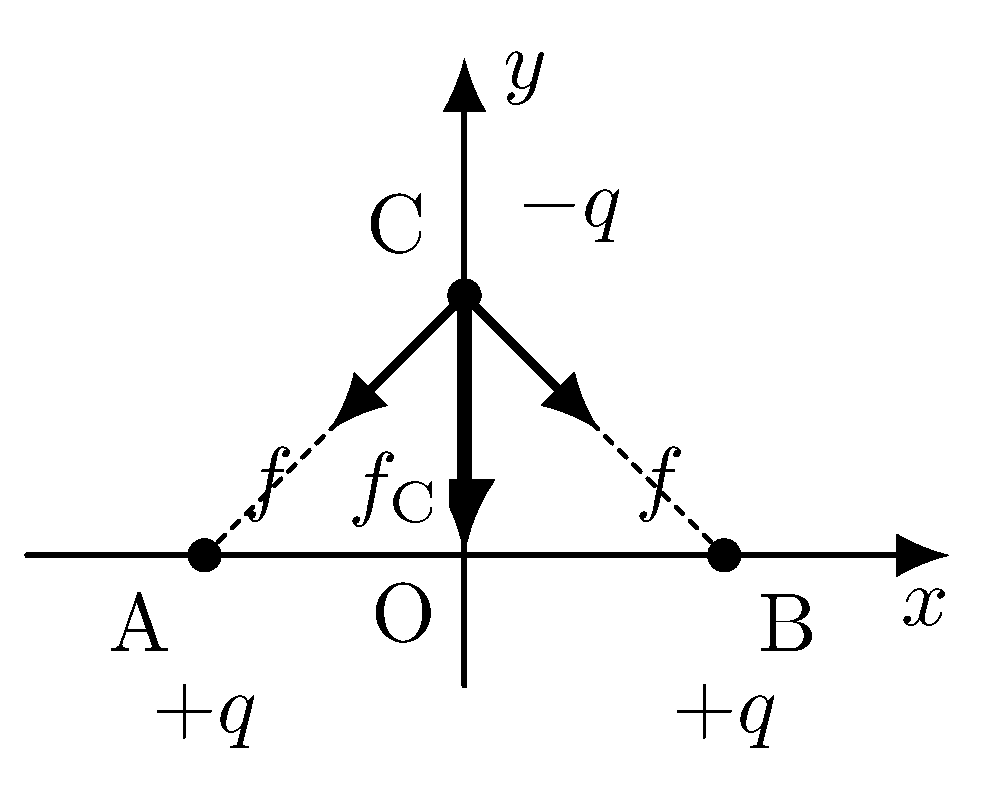
\includegraphics[keepaspectratio,width=52mm]{fig/n24_ex1_ans.png}
       \end{center}
\ko{3} (2)より$\mathrm{C}$の電荷は$-y$方向に力を受けているので，これを打ち消すには$+y$方向の力を加えればよい．$\mathrm{C}$の電荷は負であるから，正電荷は$\mathrm{C}$より{\gtfamily 上側}に置けば引力で$+y$方向に引くことができる．その位置を$(0,\ y)\ (y>d)$とすると，$\mathrm{C}$との距離は$y-d\U{m}$であるから，つり合いの式は
       \[\frac{kq^2}{(y-d)^2}=\frac{\sqrt{2}kq^2}{2d^2}\]
       これを解いて$(y-d)^2=\sqrt{2}\,d^2$，すなわち$y-d=\sqrt[4]{2}\,d$となるから，
       \Ana{\text{位置}\left(0,\ \left(1+\sqrt[4]{2}\right)d\right)\U{m}\Ans}
\end{komon}
\end{kaitou}
\end{reidaiunit}


\subsection{電場}

ある電荷が別の電荷に対して直接クーロン力を作用すると考えるのではなく，電荷を配置することによりその周辺の空間が他の電荷に力を及ぼすような状態に変化し，他の電荷はその変化した空間から力を受けると考えると便利なことが多い．
電荷が力を受けるような空間状態を{\gtfamily 電場}（電界）と呼ぶ．

クーロンの法則からわかるように電荷が受ける力は自身の電気量に比例するので，電場を，その地点に\,\AnaB{$+1\U{C}$の電荷を置いたときに受ける力}\,（ベクトル）として定義し，これを$\overrightarrow{E}$と書く．
電場が$\overrightarrow{E}$である地点に$q\U{C}$の電荷を置いたときに受ける力はその定義より
\[\overrightarrow{F}=q\overrightarrow{E}\U{N}\]
となる．

電場$\overrightarrow{E}$の大きさ$|\overrightarrow{E}|$を電場の強さと呼ぶ．
電場の単位はその定義より$\U{N/C}$である．
電場の強さが$E\U{N/C}$の点に電気量の大きさが$q\U{C}$の電荷を置くとき，電場から受ける力の大きさは
\[F=qE\U{N}\]
で与えられるが，その向きは{\gtfamily 正電荷であれば電場と同じ向き，負電荷であれば電場と逆向き}である．

\begin{matome}{電場}
 \hspace{3mm} 電場：その地点に$+1\U{C}$の電荷を置いたときに受ける力．{\gtfamily ベクトル量}\\[1mm]
 \hspace{3mm} 電場の強さが$E\U{N/C}$の点に電気量の大きさ$q\U{C}$の電荷を置くとき，受ける力の大きさは\\[0.5mm]
 \hspace{8mm} $F=qE\U{N}$\hspace{6mm}向きは{\gtfamily 正電荷なら電場と同じ向き，負電荷なら電場と逆向き}
\end{matome}

\begin{zuright}{58mm}
\hspace{1zw}電場の定義より，$q\U{C}$の点電荷が距離$r\U{m}$の点に作る電場の強さ$E\U{N/C}$は次の式で与えられる．
これは，その点に$+1\U{C}$の電荷を置いたときに受けるクーロン力の大きさ$k\dfrac{|q|\cdot 1}{r^2}$そのものである．
電場の向きは，{\gtfamily 正電荷であれば外向き，負電荷であれば内向き}である．
\zusep
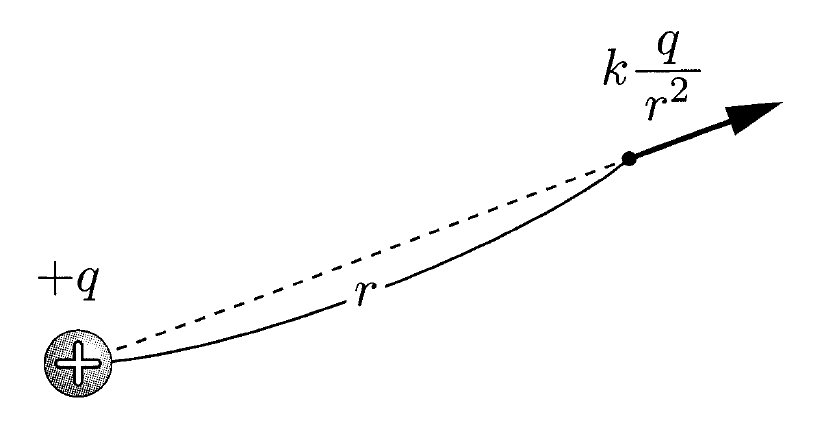
\includegraphics[keepaspectratio,width=58mm]{fig/n24_zu_ptE.png}
\end{zuright}

\AnaBD{E=k\frac{|q|}{r^2}\U{N/C}}

\noindent また，点電荷が複数ある場合には，各点電荷が単独で作る電場を{\gtfamily ベクトルとして重ね合わせれば}よい．

\begin{matome}{点電荷の作る電場}
 \hspace{3mm} $q\U{C}$の点電荷が距離$r\U{m}$の点に作る電場の強さは\hspace{3mm}$E=k\dfrac{|q|}{r^2}\U{N/C}$\\[1mm]
 \hspace{8mm} 向きは{\gtfamily 正電荷であれば外向き，負電荷であれば内向き}\\[1mm]
 \hspace{3mm} 複数の点電荷がある場合は，各点電荷が作る電場の{\gtfamily ベクトル和}
\end{matome}


%%%%%%%%%%  例題2（24.2 の直後。原本の【例題2】）  %%%%%%%%%%%%%%%%%%%%
\bsNeed{78mm}
\begin{reidaiunit}
\begin{reidai}{点電荷の作る電場}
\hspace{1zw}一直線上の$x=-r\U{m}$および$x=r\U{m}$の位置にそれぞれ$-4q\U{C}$の負電荷$\mathrm{A}$，$+q\U{C}$の正電荷$\mathrm{B}$が置かれている．クーロンの法則の比例定数を$k\U{N\cdot m^2/C^2}$として以下の設問に答えよ．ただし$q>0$とする．
\begin{center}
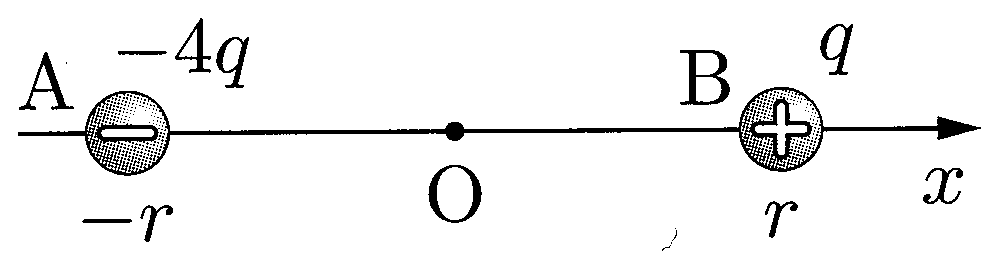
\includegraphics[keepaspectratio,width=72mm]{fig/n24_ex2_zu.png}
\end{center}
\begin{komon}
\ko{1} $\mathrm{A}$の位置に$\mathrm{B}$が作る電場の向きおよび大きさを答えよ．
\ko{2} $\mathrm{A}$が受ける力の向きおよび大きさを答えよ．
\ko{3} $x=0\U{m}$の位置に$\mathrm{A}$，$\mathrm{B}$によって作られる電場の向きおよび大きさを求めよ．
\ko{4} 無限遠方を除いて，$x$軸上で電場の大きさが$0\U{N/C}$となる点がひとつだけある．その座標を求めよ．
\end{komon}
\end{reidai}

\begin{sisinE}
複数の点電荷によって作られる電場は，各点電荷が作る電場の重ね合せとなる．大きさは$E=k\dfrac{|q|}{r^2}$で求め，向きは「正電荷なら外向き，負電荷なら内向き」で別に決める．

(4)は電場の向きを考慮するため，$x<-r$，$-r<x<r$，$r<x$に分けて考えよ．2つの電場が{\gtfamily 逆向きで大きさが等しい}ときだけ打ち消し合う．
\end{sisinE}

\Key{点電荷の作る電場の強さ\quad $E=k\dfrac{|q|}{r^2}\U{N/C}$\quad 正電荷であれば外向き，負電荷であれば内向き}

\begin{kaitou}
\begin{komon}
\ko{1} $\mathrm{B}$は正電荷であるから外向き，すなわち$\mathrm{A}$の位置では$-x$方向の電場を作る．$\overline{\mathrm{AB}}=2r\U{m}$であるから，その大きさは
       \[E=k\frac{q}{(2r)^2}=\frac{kq}{4r^2}\U{N/C}\Ans\]
       であり，向きは$-x$方向\Ans
\ko{2} $\mathrm{A}$は負電荷であるから，受ける力は電場と逆向きの$+x$方向である．\Ans\par
       その大きさは，
       \[F=|-4q|\cdot\frac{kq}{4r^2}=\frac{kq^2}{r^2}\U{N}\Ans\]
       （$\mathrm{A}$と$\mathrm{B}$は異符号ゆえ引力であり，確かに$\mathrm{B}$へ向かう向きになっている．）
\ko{3} $\mathrm{A}$が作る電場は，負電荷ゆえ$\mathrm{A}$へ向かう向き（$-x$方向）で大きさ$k\dfrac{4q}{r^2}$，$\mathrm{B}$が作る電場は，正電荷ゆえ$\mathrm{B}$から遠ざかる向き（$-x$方向）で大きさ$k\dfrac{q}{r^2}$である．向きが同じなので単純に足して，
       \[E=\frac{4kq}{r^2}+\frac{kq}{r^2}=\frac{5kq}{r^2}\U{N/C}\Ans\]
       であり，向きは$-x$方向\Ans
\ko{4} $-r<x<r$では(3)と同様に2つの電場がともに$-x$方向となり打ち消し合わない．また$x<-r$では$\mathrm{A}$の作る電場が$+x$方向，$\mathrm{B}$の作る電場が$-x$方向で逆向きになるが，電気量の大きい$\mathrm{A}$の方が近いので$\mathrm{A}$の作る電場が必ず大きく，打ち消し合わない．よって求める点は$x>r$にあり，$\mathrm{A}$の作る電場（$-x$方向）と$\mathrm{B}$の作る電場（$+x$方向）の大きさが等しいことから，
       \[k\frac{4q}{(x+r)^2}=k\frac{q}{(x-r)^2}\]
       $x>r$より$2(x-r)=x+r$であるから，
       \Ana{x=3r\U{m}\Ans}
\end{komon}
\end{kaitou}
\end{reidaiunit}


\subsection{電気力線とガウスの法則}

空間中の電場の様子を表す方法として，その接線の向きが電場の向きに一致するようになめらかに引いた曲線群を用いるという方法がある．
この曲線のことを{\gtfamily 電気力線}という．
電気力線は{\gtfamily 正電荷から出て，負電荷に入る}（もしくは無限遠方へ出入りする）．

\begin{zuright}{58mm}
\hspace{1zw}さらに，電場の強さが$E\U{N/C}$のとき電場の方向に垂直な断面の単位面積$1\U{m^2}$を貫く電気力線の本数が\,\AnaB{$E$本}\,になるように電気力線の本数を定義する．
この電気力線を用いると，電場の向きと同時に，その本数密度によって電場の強さも表すことができる．
\zusep
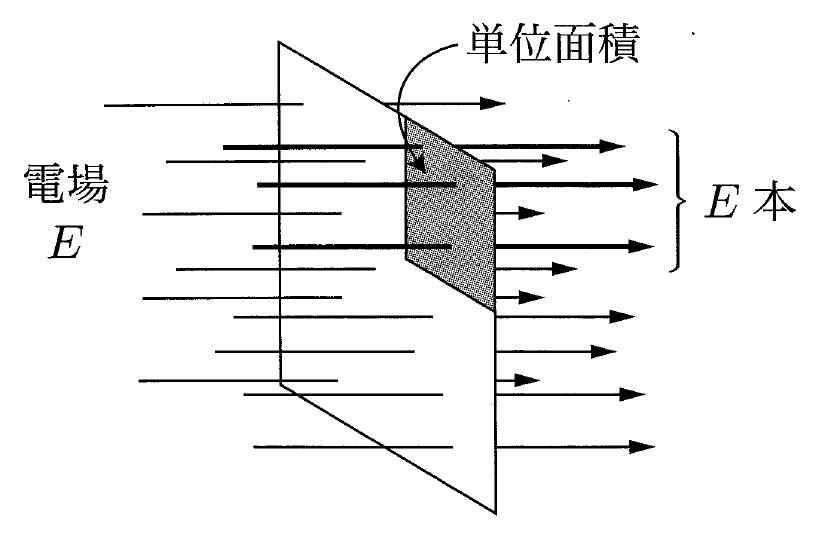
\includegraphics[keepaspectratio,width=58mm]{fig/n24_zu_lines.png}
\end{zuright}

\noindent すなわち，電気力線が{\gtfamily 密のところほど電場は強く，疎のところほど電場は弱い}．
また，電気力線は交わったり，折れ曲がったり，何もないところで途中で消えたりしない．

\begin{zuright}{46mm}
\hspace{1zw}$+q\U{C}$の電荷を中心とする半径$r\U{m}$の球面を考えると，球面における電場の強さは$k\dfrac{q}{r^2}\U{N/C}$，表面積は$4\pi r^2\U{m^2}$であるから，この球面から出ていく電気力線の本数は
\[k\frac{q}{r^2}\times 4\pi r^2=4\pi kq\]
である．
球面が大きくなると電場は弱くなるが，そのぶん表面積が広がるので，積である本数は変わらない．
\zusep
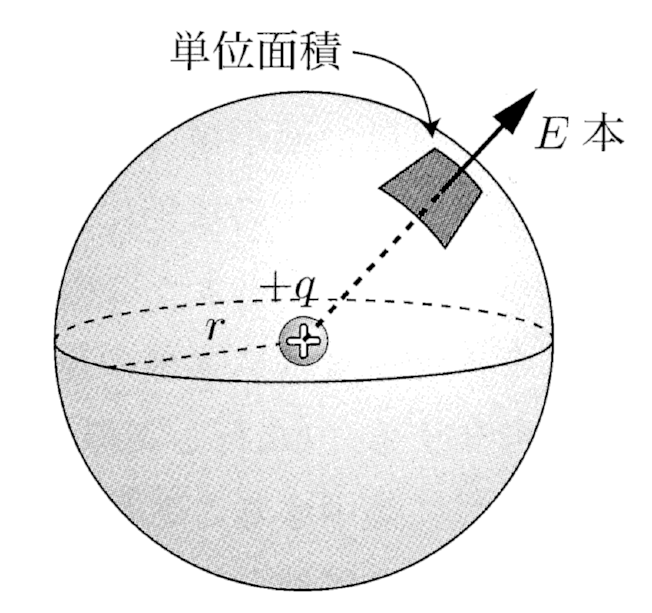
\includegraphics[keepaspectratio,width=46mm]{fig/n24_zu_gauss.png}
\end{zuright}

\noindent この本数は{\gtfamily 半径$r$によらない}ことに注意せよ．
負電荷などについても同様に考えることができ，まとめると
\AnaBD{+q\U{C}\text{の正電荷からは }4\pi kq\text{ 本の電気力線が出ていく}}
\[-q\U{C}\text{の負電荷には }4\pi kq\text{ 本の電気力線が入っていく}\]
ということが言え，これを{\gtfamily ガウスの法則}という．
すなわち，{\gtfamily 出入りする電気力線の本数は電気量だけで決まる}．
また真空の誘電率$\varepsilon_0\U{C^2/N\cdot m^2}$を用いると$k=\dfrac{1}{4\pi\varepsilon_0}$であるから，$4\pi kq=\dfrac{q}{\varepsilon_0}$と書き換えることもできる．

\begin{matome}{電気力線とガウスの法則}
 \hspace{3mm} 電気力線：{\gtfamily 接線方向}は電場の向きを，{\gtfamily 本数密度}は電場の強さを表す\\[1mm]
 \hspace{8mm} $+q\U{C}$の正電荷からは$4\pi kq$本の電気力線が出ていく\\[0.5mm]
 \hspace{8mm} $-q\U{C}$の負電荷には$4\pi kq$本の電気力線が入っていく\\[1mm]
 \hspace{3mm} 電気力線は途中で交わったり，折れ曲がったり，途中で消えたりしない
\end{matome}

電気力線のおおまかな様子は慣れると直感的にわかり，電場の様子を簡単に把握できる．

%%%%%%%%%%  例題3（24.3 の直後。原本の【例題3】）  %%%%%%%%%%%%%%%%%%%%
\bsNeed{74mm}
\begin{reidaiunit}
\begin{reidai}{電気力線}
\begin{zuright}{52mm}
\hspace{1zw}一辺の長さが$a\U{m}$の正三角形の頂点に3個の点電荷$\mathrm{A}$，$\mathrm{B}$，$\mathrm{C}$が固定されており，それぞれ$-2Q\U{C}$，$Q\U{C}$，$Q\U{C}$の電気量を持つ．図のように，$\mathrm{A}$を原点とし，辺$\mathrm{BC}$が$x$軸と垂直になるように座標軸を取る．$Q>0$，クーロンの比例定数を$k\U{N\cdot m^2/C^2}$とし，この$xy$平面内では$\mathrm{B}$，$\mathrm{C}$の電荷からは6本の電気力線が出ているものとして以下の設問に答えよ．
\zusep
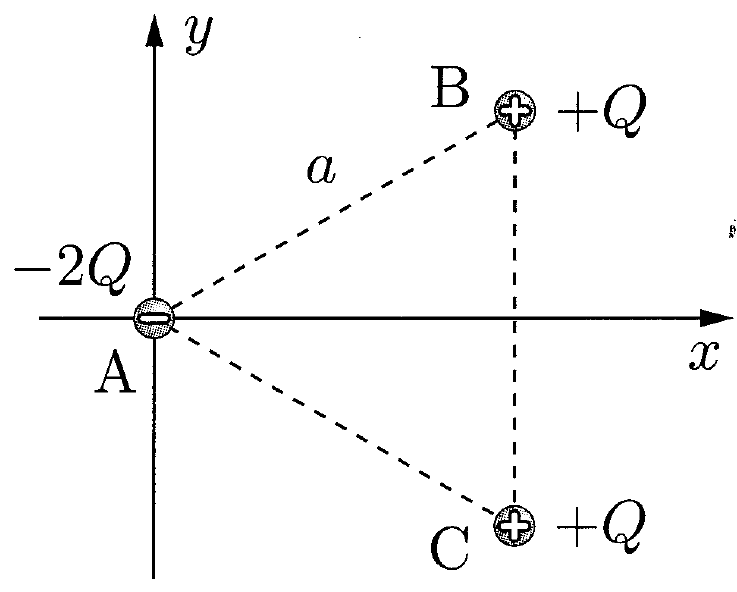
\includegraphics[keepaspectratio,width=52mm]{fig/n24_ex3_zu.png}
\end{zuright}
\begin{komon}
\ko{1} $\mathrm{A}$がなく，$\mathrm{B}$，$\mathrm{C}$のみが配置されている場合の電気力線の$xy$平面内の大体の様子を図示せよ．
\ko{2} $\mathrm{A}$，$\mathrm{B}$，$\mathrm{C}$の3つの点電荷によって作られる電気力線の$xy$平面内の大体の様子を図示せよ．
\end{komon}
\end{reidai}

\begin{sisinE}
電気力線は{\gtfamily 正電荷から出て負電荷に入る}のであり，途中で交わったり枝分かれしたりしない．この2点だけで大体の様子は決まる．

本数に着目するのがこの問題の要である．$Q\U{C}$から6本出るのだから，$-2Q\U{C}$には$12$本入る．すなわち$\mathrm{B}$，$\mathrm{C}$から出る合計$12$本は{\gtfamily すべて$\mathrm{A}$に入ってしまい，無限遠方へ逃げる電気力線は1本も無い}．
\end{sisinE}

\Key{$+q\U{C}$の正電荷からは$4\pi kq$本が出て，$-q\U{C}$の負電荷には$4\pi kq$本が入る（本数は電気量だけで決まる）}

\begin{kaitou}
\begin{komon}
\ko{1} 同符号の2電荷であるから電気力線は互いに反発するように広がり，$\mathrm{BC}$の中点付近では電場が打ち消し合って$0$になる．出た$12$本はすべて無限遠方へ逃げる．
       \begin{center}\AnaFig{58mm}{fig/n24_ex3_ans1.png}{fig/n24_ex3_ans1_blank.png}\end{center}
       \hspace*{\fill}\Ans
\ko{2} $\mathrm{B}$，$\mathrm{C}$から出る電気力線は$6+6=12$本，$\mathrm{A}$に入る電気力線は$4\pi k\cdot 2Q$本，すなわち$12$本である．よって{\gtfamily $\mathrm{B}$，$\mathrm{C}$から出た電気力線はすべて$\mathrm{A}$に入り}，無限遠方へ出ていく電気力線は無い．
       \begin{center}\AnaFig{58mm}{fig/n24_ex3_ans2.png}{fig/n24_ex3_ans2_blank.png}\end{center}
       \hspace*{\fill}\Ans
\end{komon}
\end{kaitou}
\end{reidaiunit}


\subsection{静電誘導と導体の性質}

\begin{zuright}{50mm}
\hspace{1zw}電子の移動・過不足により電気量を持つ電荷が生じるが，同種の電荷同士はクーロンの法則により互いに反発しあうため，帯電体の電荷はなるべく拡散するように物質中もしくは物質表面に分布する．
また，逆にそばに異種の電荷がある場合はそれになるべく近づくように分布する．
\zusep
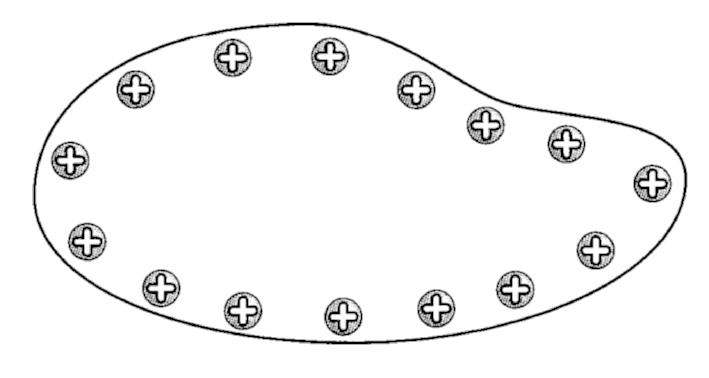
\includegraphics[keepaspectratio,width=50mm]{fig/n24_zu_bunpu.png}
\end{zuright}

\noindent （ただし，実際には同種の電荷同士の反発もあるため，電荷が一点に集中することはない．）

金属は，金属結合により自由電子が内部で自由に動ける性質を持つ．
そのため，金属に正の帯電体を近づけると，帯電体に近い側には電子が集まって負に帯電し，逆に帯電体から遠い側では電子が不足して正に帯電する．
また，金属に負の帯電体を近づけると，帯電体に近い側からは電子が逃げて正に帯電し，逆に帯電体から遠い側では電子が集まって負に帯電する．
このような現象を\,\AnaB{静電誘導}\,と呼ぶが，これは以上で述べたように，電荷同士の斥力・引力および電荷分布を考えることにより説明できる．
% 加筆（2026-09-23）：実際に動くのは電子だけである，という確認を本文に上げた．
%   練習［39］［40］の解答がこれを前提にしている（原本は指針にしか書いていない）．
なお，{\gtfamily 実際に物体間を移動するのは電子だけ}であり，正電荷を持つ陽イオンは動かない．「正に帯電した」とは電子が不足したという意味である．

\begin{matome}{電荷の振る舞い}
 \hspace{3mm} 同種の電荷同士は反発しあい，可能な限り拡散しようとする\\[1mm]
 \hspace{3mm} 異種の電荷同士は引き合い，なるべく近づこうとする\\[1mm]
 \hspace{3mm} 実際に移動するのは{\gtfamily 電子}だけである
\end{matome}

金属のように電気をよく通すものを{\gtfamily 導体}と呼び，逆にプラスチックのように電気を通さないものを{\gtfamily 不導体}（もしくは{\gtfamily 誘電体}）と呼ぶ．

\begin{zuright}{52mm}
\hspace{1zw}導体，例えば金属の場合，その自由電子は金属内を自由に動き回れるため，電子が導体内で動くのにエネルギーを必要としない．
このことから，{\gtfamily 導体内の電位は一定}である（電位については24.5で述べる）．
また，導体に外部から電場がかけられるとその電場によって速やかに電子が移動し，外部からかけられた電場を打ち消すことにより電子の移動が止まる．
\zusep
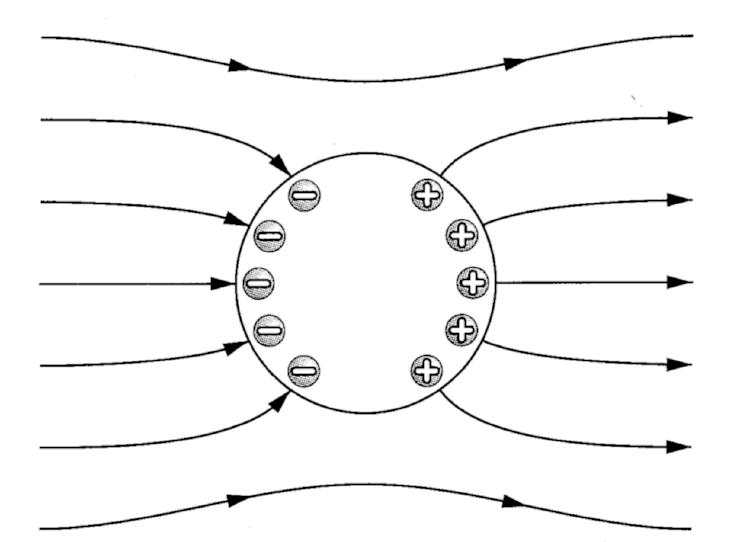
\includegraphics[keepaspectratio,width=52mm]{fig/n24_zu_doutai.png}
\end{zuright}

\noindent そのため，外部から{\gtfamily 電場をかけても導体内には電場が生じない}．

また，静電状態（電流が流れていない状態）の導体内部にもし電荷があると導体内部に電場が生じてしまうが，これは上で述べたことに反する．
よって，{\gtfamily 静電状態にある導体の内部には電荷が生じず，導体表面に電荷が現れる}．

この性質を利用すると，例えば図(a)のように箔検電器を接地した金属製の箱で囲むことにより，外部から帯電したエボナイト棒を近づけても静電誘導は起こらない．
また図(b)のように帯電した物体を接地した金属製の箱で覆うことにより，帯電体から出てくる電場を遮断することができる．
このように，導体で囲むことによって内外の電場を遮断することを\,\AnaB{静電遮蔽}\,という．

\begin{center}
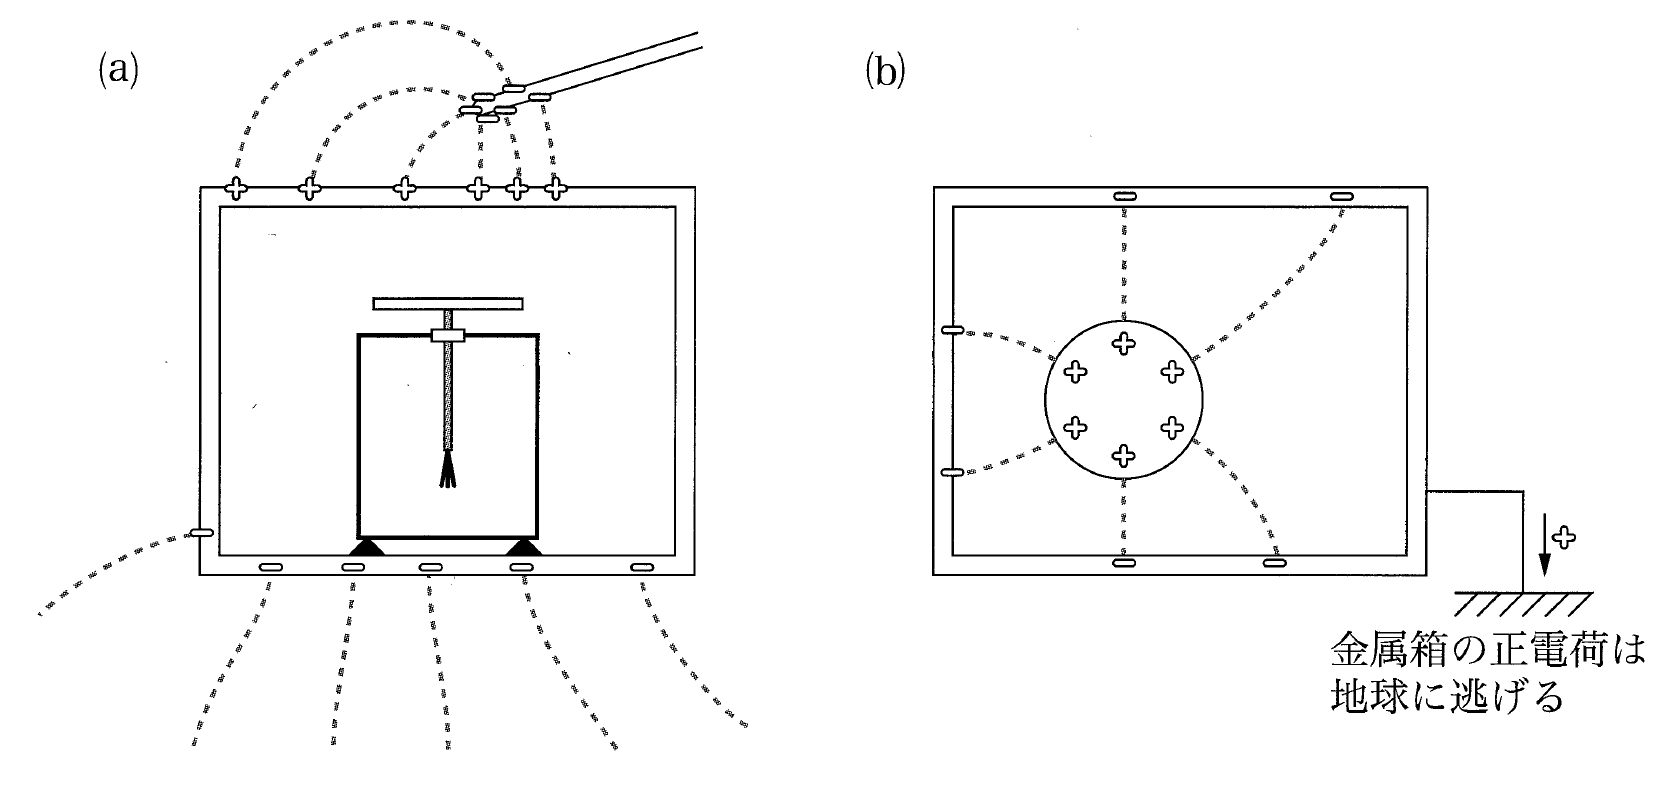
\includegraphics[keepaspectratio,width=118mm]{fig/n24_zu_shahei.png}
\end{center}

\begin{matome}{導体の性質}
 \hspace{3mm} 導体内の{\gtfamily 電位は一定}（＝導体内に電場は生じない）\\[1mm]
 \hspace{3mm} 静電状態の導体の{\gtfamily 内部に電荷は無く，表面にだけ電荷が現れる}\\[1mm]
 \hspace{3mm} 導体で囲むと内外の電場を遮断できる（{\gtfamily 静電遮蔽}）
\end{matome}


\subsection{電位と一様電場}

空間中の電場の様子を表す方法として，電気力線を使う方法の他に，電位というものを利用する方法がある．
この電位を利用すると，電場が荷電粒子に対してなす仕事を考えることができる．

\begin{zuright}{46mm}
\hspace{1zw}$+1\U{C}$の点電荷を，電場に逆らって$\mathrm{O}$点（基準点）からゆっくり$\mathrm{P}$点まで動かすのに必要な仕事（エネルギー）が$V\U{J}$であるとき，$\mathrm{P}$点の{\gtfamily 電位}を$V\U{V}$（ボルト）と定義する．
この電位を利用すると，$+q\U{C}$の電荷を基準点$\mathrm{O}$から電位$V\U{V}$の点までゆっくりと動かすためには$qV\U{J}$のエネルギーが必要である，と言える．\par
\hspace{1zw}電位の基準点は，基本的にどこに取ってもよいが，{\gtfamily 無限遠方}，もしくは回路の問題では{\gtfamily 接地されている点}（アース）を基準点に取ることが多い．
\zusep
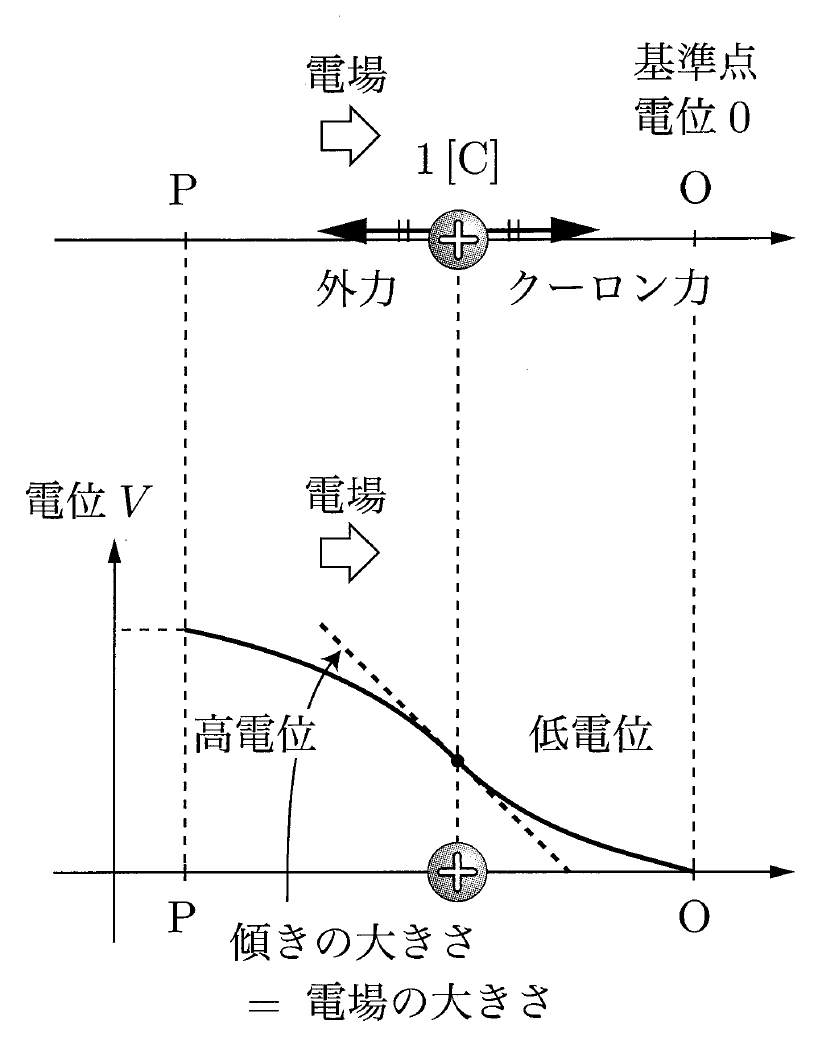
\includegraphics[keepaspectratio,width=46mm]{fig/n24_zu_deni.png}
\end{zuright}

\noindent 以上のことから，$+q\U{C}$の電荷が電位$V\U{V}$の点で持つ位置エネルギーは

\AnaBD{U=qV\U{J}}

\noindent である．

\begin{matome}{電荷の持つ位置エネルギー}
 \hspace{3mm} $+q\U{C}$の点電荷が$V\U{V}$の電位の点で持つ位置エネルギーは\hspace{3mm}$U=qV\U{J}$
\end{matome}

この電位を用いて電場を考えると，{\gtfamily 電場は電位の大きい方から小さい方へと向かっている}ので，電位は電荷にとっての高さのようなものだと考えればよい．
すなわち，{\gtfamily 正電荷は}\,\AnaB{高電位$\rightarrow$低電位}\,{\gtfamily へ向かおうとし，負電荷は低電位$\rightarrow$高電位へと向かおうとする}．
また，電位の傾きが大きいほど受ける力は大きいので，{\gtfamily 電位の傾きが電場の大きさに対応している}．

% 加筆（2026-09-23）：等電位面の定義と「電場は等電位面に直交する」を本文へ上げた．
%   原本は例題5の指針で初出だったが，例題4(2)・練習［45］［46］がこれを使う．
電位が等しい点を連ねた面（平面内で考えるときは線）を{\gtfamily 等電位面}（{\gtfamily 等電位線}）という．
等電位面に沿って電荷を動かしても仕事は$0$であるから，{\gtfamily 電場（電気力線）は等電位面に必ず直交する}．
また電位の傾きが電場の大きさであったから，{\gtfamily 等電位面の間隔が狭いところほど電場が強い}．

電場の様子に応じてさまざまな電位が存在するが，そのうち以下の2つを覚えておけば十分である．

\hspace{1zw}$\MARU{1}$\hspace{2mm}{\gtfamily 一様電場}\par
\hspace{1zw}2つの金属板を距離$d\U{m}$だけ離して平行に配置し（これを{\gtfamily 平行平板コンデンサー}という），各々を$+Q\U{C}$，$-Q\U{C}$に帯電させると，図の$\mathrm{A}\rightarrow\mathrm{B}$へと向かう，平行かつ一様な電場$E\U{N/C}$が生じる．図から明らかに正に帯電した$\mathrm{A}$側がより高電位となる．
$V$-$x$グラフの傾きが$E$であるから，$\mathrm{A}$と$\mathrm{B}$の電位差は

\begin{center}
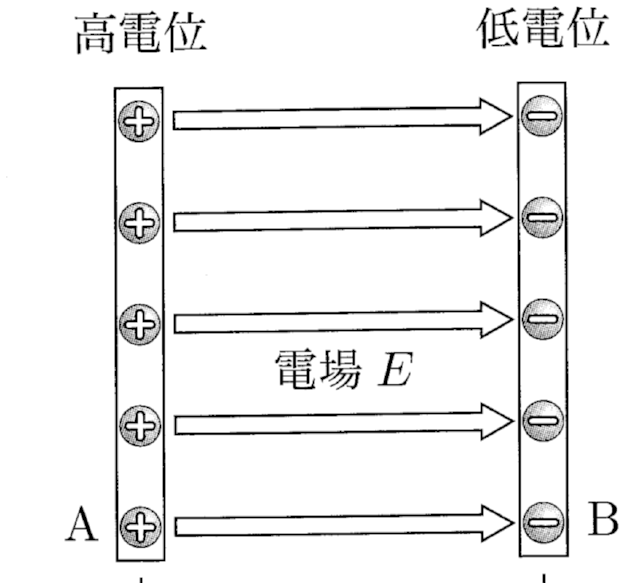
\includegraphics[keepaspectratio,width=44mm]{fig/n24_zu_ichiyou.png}\hspace{12mm}
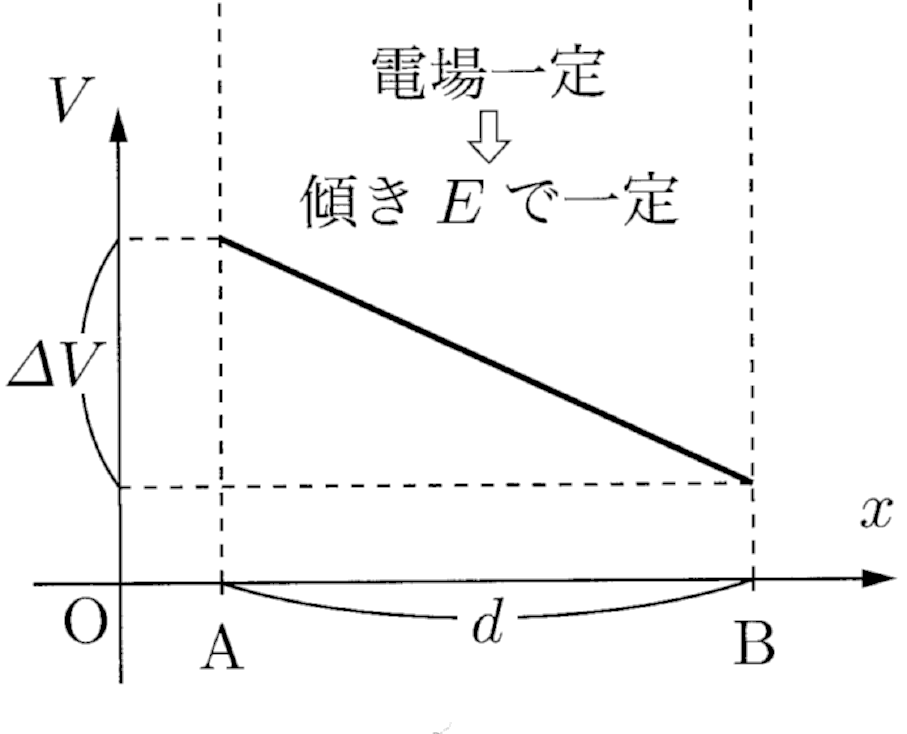
\includegraphics[keepaspectratio,width=64mm]{fig/n24_zu_ichiyouV.png}
\end{center}

\AnaBD{\Delta V=Ed\U{V}}

\noindent で与えられる．
すなわち，{\gtfamily 負に帯電した金属板よりも正に帯電した金属板の方が$Ed\U{V}$だけ電位が高い}．

$\MARU{1}$のグラフから分かるように，向きまで考慮すると電場と電位との間には，
\AnaBD{E=-\frac{dV}{dx}\U{N/C}}
の関係がある．
この式から，電場の単位は$\U{N/C}=\U{V/m}$である．

\begin{matome}{電場と電位}
 \hspace{3mm} $E=-\dfrac{dV}{dx}\U{N/C}$\hspace{6mm}電場は{\gtfamily 高電位$\rightarrow$低電位}を向く\\[1mm]
 \hspace{3mm} {\gtfamily 電位の傾きの大きさが電場の大きさ}．一様電場では$\Delta V=Ed\U{V}$\\[1mm]
 \hspace{3mm} 電場（電気力線）は{\gtfamily 等電位面に直交する}．等電位面が密なところほど電場は強い
\end{matome}

%%%%%%%%%%  例題4（24.5 の直後。原本の【例題5】）  %%%%%%%%%%%%%%%%%%%%
\bsNeed{96mm}
\begin{reidaiunit}
\begin{reidai}{一様電場による電位}
\begin{zuright}{76mm}
\hspace{1zw}真空中に図のような平行な2枚の金属板$\mathrm{X}$，$\mathrm{Y}$が距離$d\U{m}$だけ隔てて置いてあり，$\mathrm{X}$，$\mathrm{Y}$間には$\mathrm{X}$が高電位となるように大きさ$V\U{V}$の電圧がかけられている．重力を無視してよいものとし，極板は$d\U{m}$に比べて十分大きいものとして以下の設問に答えよ．
\zusep
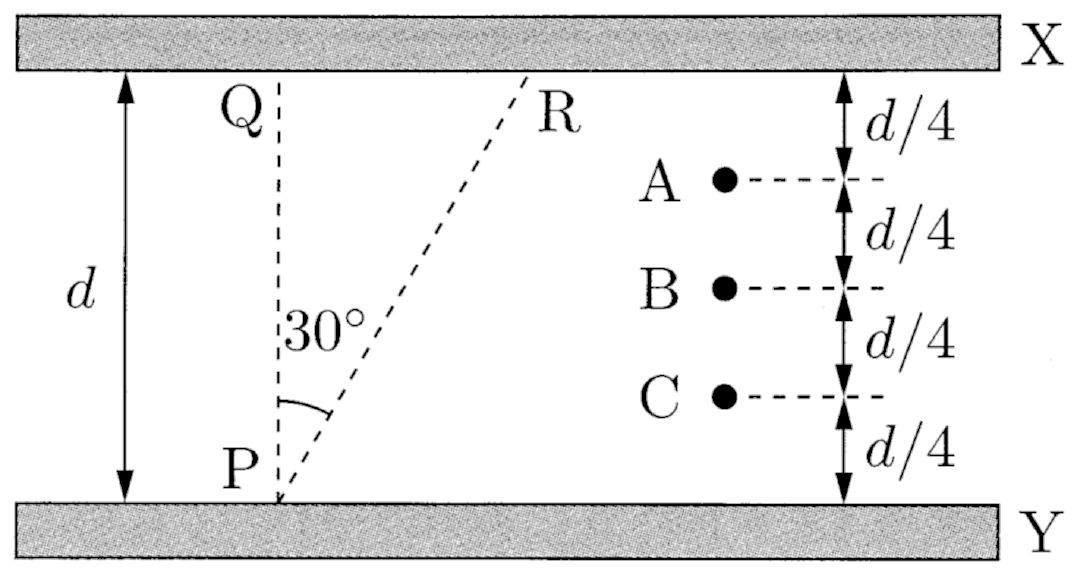
\includegraphics[keepaspectratio,width=76mm]{fig/n24_ex4_zu.png}
\end{zuright}
\begin{komon}
\ko{1} 金属板$\mathrm{X}$，$\mathrm{Y}$の間に生じる電場の向きと強さをそれぞれ求め，その様子を電気力線を用いて実線で図示せよ．
\ko{2} 金属板$\mathrm{X}$，$\mathrm{Y}$の間の等電位面はどのようになるか．点線で図示せよ．
\ko{3} 金属板$\mathrm{Y}$の電位を基準$0\U{V}$とするとき，金属板間を4等分した図の$\mathrm{A}$，$\mathrm{B}$，$\mathrm{C}$点の電位をそれぞれ求めよ．
\ko{4} 正の電荷$+q\U{C}$をこの金属板間に置くとき，受ける力の向きおよび大きさをそれぞれ求めよ．
\ko{5} この正電荷を図の点線に沿ってゆっくりと$\mathrm{P}$点から$\mathrm{Q}$点まで運ぶのに要する仕事と，ゆっくりと$\mathrm{P}$点から$\mathrm{R}$点まで運ぶのに要する仕事をそれぞれ求めよ．
\ko{6} 負電荷$-q\U{C}$を持つ質量$m\U{kg}$の点電荷を$\mathrm{P}$点に置くと，この点電荷は電場によって$\mathrm{Q}$点に達する．点電荷が$\mathrm{P}$点を初速$0\U{m/s}$で出発した場合，この点電荷が$\mathrm{Q}$点に達したときの速さを求めよ．
\end{komon}
\end{reidai}

\begin{sisinE}
電圧とは，2点間の電位差のことをいう．電位と電場の様子をグラフに書きながら考えよ．

(2) 等電位面とは電位が等しくなる点を連ねた面（二次元の場合は線）であり，電場は必ず等電位面（等電位線）に対して直交する．本問の等電位面が極板に平行な面になることが分かれば，(5)で$\mathrm{Q}$と$\mathrm{R}$が同電位であることも見える．
\end{sisinE}

\Key{一様電場：$\Delta V=Ed$\quad 電気力線は高電位の極板から低電位の極板へ向かう平行線，等電位面はそれに直交}

\begin{kaitou}
\begin{komon}
\ko{1} $\mathrm{X}$が高電位であるから電場は$\mathrm{X}\rightarrow\mathrm{Y}$の向き（鉛直下向き）であり，その強さは$\Delta V=Ed$より
       \[E=\frac{V}{d}\U{V/m}\Ans\]
\ko{2} 電気力線に直交するから，{\gtfamily 極板に平行な面}になる．(1)とあわせて図示すると次図（実線が電気力線，点線が等電位面）．
       \begin{center}\AnaFig{86mm}{fig/n24_ex4_ans.png}{fig/n24_ex4_ans_blank.png}\end{center}
       \hspace*{\fill}\Ans
\ko{3} 一様電場であるから電位は$\mathrm{Y}$からの距離に比例する．$\mathrm{A}$，$\mathrm{B}$，$\mathrm{C}$の$\mathrm{Y}$からの距離はそれぞれ$\dfrac{3}{4}d$，$\dfrac{1}{2}d$，$\dfrac{1}{4}d\U{m}$であるから，
       \[V_{\mathrm{A}}=\frac{3}{4}V,\quad V_{\mathrm{B}}=\frac{1}{2}V,\quad V_{\mathrm{C}}=\frac{1}{4}V\U{V}\Ans\]
\ko{4} 正電荷が受ける力の向きは電場と同じ向き，すなわち$\mathrm{X}\rightarrow\mathrm{Y}$の向き\Ans\par
       大きさは
       \[F=qE=\frac{qV}{d}\U{N}\Ans\]
\ko{5} $\mathrm{P}$は$\mathrm{Y}$上の点だから$V_{\mathrm{P}}=0\U{V}$，$\mathrm{Q}$，$\mathrm{R}$はいずれも$\mathrm{X}$上の点だから$V_{\mathrm{Q}}=V_{\mathrm{R}}=V\U{V}$である．ゆっくり運ぶので運動エネルギーは変化せず，外力のした仕事はすべて位置エネルギーの変化になる．よっていずれも
       \[W=q(V-0)=qV\U{J}\Ans\]
       \begin{chuu}
       $\mathrm{Q}$と$\mathrm{R}$は同一の等電位面上にあるので，経路の長さが違っても必要な仕事は同じである．静電気力は{\gtfamily 保存力}であり，その仕事は始点と終点だけで決まる．
       \end{chuu}
\ko{6} 負電荷$-q\U{C}$の$\mathrm{P}$点での位置エネルギーは$(-q)\cdot 0=0\U{J}$，$\mathrm{Q}$点での位置エネルギーは$(-q)\cdot V=-qV\U{J}$である．力学的エネルギー保存則より，
       \[0+0=\frac{1}{2}mv^2+(-qV)\]
       であるから，
       \[v=\sqrt{\frac{2qV}{m}}\U{m/s}\Ans\]
\end{komon}
\end{kaitou}
\end{reidaiunit}


\subsection{点電荷による電位}

\begin{zuright}{54mm}
\hspace{1zw}$\MARU{2}$\hspace{2mm}{\gtfamily 点電荷による電位}\par
\hspace{1zw}原点に$+Q\U{C}$の点電荷が置かれているとき，座標$x\U{m}\ (>0)$における電場は$+x$方向に$E=k\dfrac{Q}{x^2}\U{N/C}$であるから，この点において$\dfrac{d}{dx}V(x)=-k\dfrac{Q}{x^2}$を満たすような$V(x)\U{V}$が電位である．
\zusep
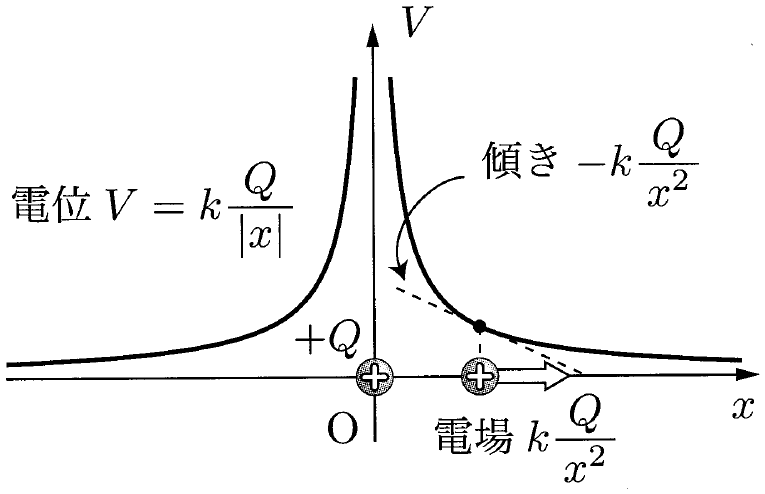
\includegraphics[keepaspectratio,width=54mm]{fig/n24_zu_ptV.png}
\end{zuright}

\noindent よって，この式の両辺を積分すると，
\[V(x)=-\int k\frac{Q}{x^2}\,dx=k\frac{Q}{x}+C\]
となるが，この積分定数$C$の値は，電位の基準点をどこにするかによって決まる．
式が簡単になるように，{\gtfamily 無限遠点を基準にする}，すなわち$x\rightarrow\infty$のとき$V(x)\rightarrow 0$となるように$C$の値をとると，
\[V(x)=k\frac{Q}{x}\U{V}\]
と表される．$x<0$の場合も含めると$V(x)=k\dfrac{Q}{|x|}\U{V}$となり，点電荷からの距離を$r\U{m}$とすれば
\AnaBD{V=k\frac{Q}{r}\U{V}}
となる．
{\gtfamily この式には電気量$Q$を符号ごと代入する}（負電荷の作る電位は負になる）．電場の式$E=k\dfrac{|q|}{r^2}$が絶対値であったのと対照的なので混同しないこと．

また，点電荷が複数ある場合には，その重ね合わせで電位を求めればよい．
% 加筆（2026-09-23）：電位がスカラーであることを明示した．練習［43］［45］［46］の要．
電場はベクトルなので向きを考えてベクトル和を取らねばならなかったが，{\gtfamily 電位はスカラーであるから向きを考える必要がなく}，\,\AnaB{単純和}\,を取ればよい．

\begin{matome}{一様電場・点電荷による電位}
\begin{description}
\item[\MARU{1}] {\gtfamily 一様電場による電位}\\
強さ$E\U{N/C}$，距離$d\U{m}$離れた2点間の電位差は\hspace{3mm}$\Delta V=Ed\U{V}$
\item[\MARU{2}] {\gtfamily 点電荷による電位}\\
$Q\U{C}$の点電荷から距離$r\U{m}$の点における電位は無限遠点を基準として\hspace{3mm}$V=k\dfrac{Q}{r}\U{V}$\\[0.5mm]
（$Q$は{\gtfamily 符号ごと}代入する．複数あるときは{\gtfamily 単純和}）
\end{description}
\end{matome}

%%%%%%%%%%  例題5（24.6 の直後。原本の【例題6】）  %%%%%%%%%%%%%%%%%%%%
\bsNeed{72mm}
\begin{reidaiunit}
\begin{reidai}{点電荷による電位}
\hspace{1zw}$x$軸上で$r\U{m}$離れた2点$\mathrm{A}$，$\mathrm{B}$に，図のように電気量がそれぞれ$+3q\U{C}$，$-q\U{C}$の点電荷を置いた．$\mathrm{A}$点を$x$軸の原点$\mathrm{O}$とし，無限遠方を電位の基準点とする．クーロンの比例定数を$k\U{N\cdot m^2/C^2}$として以下の設問に答えよ．ただし$q>0$とする．
\begin{center}
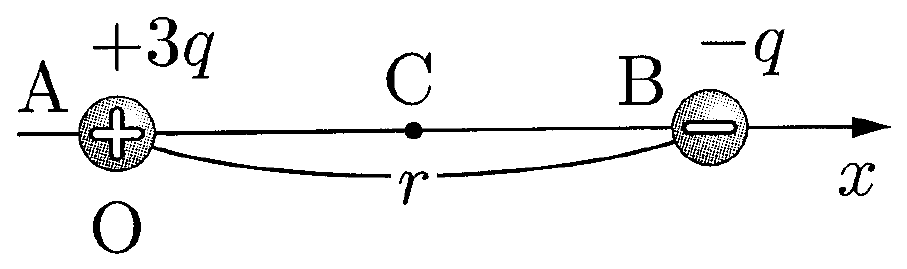
\includegraphics[keepaspectratio,width=64mm]{fig/n24_ex5_zu.png}
\end{center}
\begin{komon}
\ko{1} 2点$\mathrm{A}$，$\mathrm{B}$の中点$\mathrm{C}$における電場を求めよ．
\ko{2} 中点$\mathrm{C}$における電位を求めよ．
\ko{3} $x$軸上で電位が無限遠方の他に$0\U{V}$となる点を求めよ．
\end{komon}
\end{reidai}

\begin{sisinE}
座標計算をする際には，点電荷の右側と左側で点電荷からの距離$r\U{m}$の表式が異なることに注意せよ．一般には$|x-x_0|$と絶対値で書いておき，最後に場合分けして外す．

電場は{\gtfamily 絶対値を代入して大きさを求め向きは別に考える}，電位は{\gtfamily 符号ごと代入して単純和}，という違いをはっきり意識すること．
\end{sisinE}

\Key{$Q\U{C}$の点電荷から距離$r\U{m}$の点における電位は無限遠方を基準として\quad $V=k\dfrac{Q}{r}\U{V}$}

\begin{kaitou}
\begin{komon}
\ko{1} $\mathrm{C}$は$\mathrm{A}$，$\mathrm{B}$のいずれからも$\dfrac{r}{2}\U{m}$の距離にある．$\mathrm{A}$の作る電場は正電荷ゆえ外向き（$+x$方向）で大きさ$k\dfrac{3q}{(r/2)^2}=\dfrac{12kq}{r^2}$，$\mathrm{B}$の作る電場は負電荷ゆえ内向き（$+x$方向）で大きさ$k\dfrac{q}{(r/2)^2}=\dfrac{4kq}{r^2}$である．向きが同じであるから，
       \[E=\frac{12kq}{r^2}+\frac{4kq}{r^2}=\frac{16kq}{r^2}\U{N/C}\Ans\]
       であり，向きは$+x$方向（$\mathrm{A}\rightarrow\mathrm{B}$の向き）\Ans
\ko{2} 電位は符号ごと代入して単純和を取ればよいから，
       \[V_{\mathrm{C}}=k\frac{+3q}{r/2}+k\frac{-q}{r/2}=\frac{6kq}{r}-\frac{2kq}{r}=\frac{4kq}{r}\U{V}\Ans\]
\ko{3} $x$軸上の点の座標を$x\U{m}$とすると，$\mathrm{A}$からの距離は$|x|$，$\mathrm{B}$からの距離は$|x-r|$であるから，
       \[V(x)=k\frac{3q}{|x|}+k\frac{-q}{|x-r|}=0\]
       すなわち$3|x-r|=|x|$である．$x<0$では$3(r-x)=-x$より$x=\dfrac{3}{2}r>0$となり不適，$0<x<r$では$3(r-x)=x$より$x=\dfrac{3}{4}r$，$x>r$では$3(x-r)=x$より$x=\dfrac{3}{2}r$である．よって，
       \Ana{x=\frac{3}{4}r,\quad \frac{3}{2}r\U{m}\Ans}
       \begin{chuu}
       {\gtfamily 電位が$0$になる点と電場が$0$になる点とは別}である（電場が$0$になるのは$\mathrm{B}$の右側の1点だけ）．
       \end{chuu}
\end{komon}
\end{kaitou}
\end{reidaiunit}

\newpage

%%%%%%%%%%%%%%%%%%%%  練習問題  %%%%%%%%%%%%%%%%%%%%
% 第23回の［33］に続く．章単体で組んだときも番号が本体と一致するように明示しておく
\setcounter{qno}{33}

\filbreak
\Rank{A問題}

% A問題の統合：旧㉙[1]（(1)(2)(3)）と旧㉚[8]（(1)(2)(3)）を1題にまとめた．
%   設問は1つも失われていない．
\Mon{基本公式の確認}

\hspace{1zw}以下の設問に答えよ．ただし，クーロンの法則の比例定数を$k=9.0\times 10^9\U{N\cdot m^2/C^2}$とする．
\begin{komon}
\ko{1} 真空中で$100\U{m}$だけ隔てて$+1.0\U{C}$と$-4.0\U{C}$の電荷がある．その間に働く静電気力の大きさは何$\U{N}$か．
\ko{2} 真空中に$+7.0\times 10^{-8}\U{C}$の点電荷が置かれている．この点電荷から$0.30\U{m}$だけ離れた点$\mathrm{A}$での電場の強さは何$\U{N/C}$か．またどちら向きか．
\ko{3} ある点に$-4.0\times 10^{-8}\U{C}$の点電荷を置いたところ，この電荷は右向きに大きさ$8.0\times 10^{-5}\U{N}$の力を受けた．この点における電場の強さは何$\U{N/C}$か．またどの向きか．
\ko{4} 強さ$3.0\U{V/m}$の一様な電場に沿って，$1.5\U{m}$だけ離れた2点間の電位差は何$\U{V}$か．
\ko{5} $-5.6\times 10^{-6}\U{C}$の点電荷が，$2.0\U{m}$だけ離れた点に作る電位は何$\U{V}$か．ただし，電位の基準点を無限遠方とする．
\ko{6} $+0.25\U{C}$の点電荷を点$\mathrm{A}$から点$\mathrm{B}$へゆっくりと移動させるのに，外力のした仕事は$8.0\U{J}$であった．$\mathrm{AB}$間の電位差は何$\U{V}$か．また点$\mathrm{A}$，$\mathrm{B}$のいずれの点の電位が高いか．
\end{komon}

\filbreak
\Rank{B問題}

\Mon{クーロンの法則}

\hspace{1zw}電荷のわかっていない三つの点電荷$\mathrm{A}$，$\mathrm{B}$，$\mathrm{C}$がある．$\mathrm{A}$と$\mathrm{B}$を$r\U{m}$だけ離しておくと，その間に働く力は大きさ$f_1\U{N}$の引力，$\mathrm{B}$と$\mathrm{C}$を$r\U{m}$だけ離しておくと，その間に働く力は大きさ$f_2\U{N}$の斥力，$\mathrm{C}$と$\mathrm{A}$を$r\U{m}$だけ離しておくと，その間に働く力は大きさ$f_3\U{N}$の引力が働いた．クーロンの法則の比例定数を$k\U{N\cdot m^2/C^2}$として$\mathrm{A}$，$\mathrm{B}$，$\mathrm{C}$の電荷を求めよ．ただし，$\mathrm{B}$の電荷は負であることがわかっている．

\Mon{クーロンの法則と力のつり合い}

\begin{zuright}{40mm}
\hspace{1zw}質量がともに$m\U{kg}$で等しい大きさの電荷を持つ二つの小球を，長さ$l\U{m}$の二本の絹糸で同じ場所からつり下げたところ，糸が鉛直線と角度$\theta$をなす場所でつり合った．クーロンの法則の比例定数を$k\U{N\cdot m^2/C^2}$，重力加速度の大きさを$g\U{m/s^2}$として以下の設問に答えよ．
\begin{komon}
\ko{1} 二つの電荷の符号は同符号，異符号のいずれか．
\ko{2} 小球の持つ電荷の大きさを$q\U{C}$，糸の張力の大きさを$T\U{N}$として，小球間に作用するクーロン力，重力，張力の力のつり合いの式を示せ．
\ko{3} 小球の持つ電荷の大きさを求めよ．
\end{komon}
\zusep
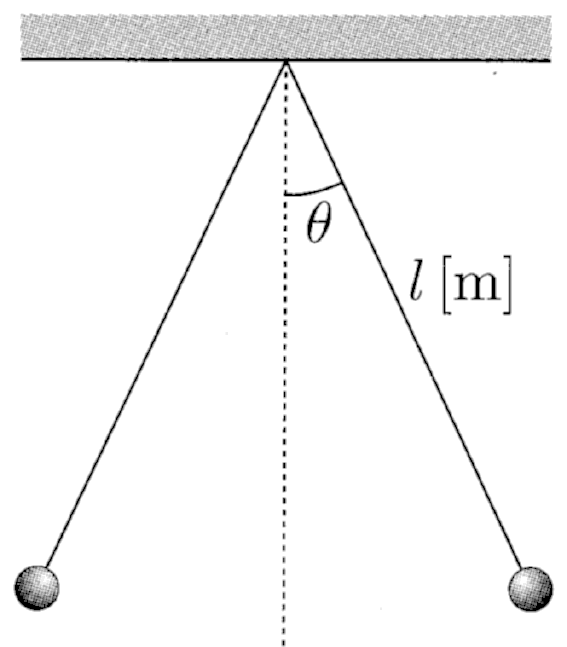
\includegraphics[keepaspectratio,width=40mm]{fig/n24_p36_zu.png}
\end{zuright}

\Mon[\Sitei]{クーロン力と電場}

\begin{zuright}{52mm}
\hspace{1zw}右図のように，原点$\mathrm{O}$からともに距離$d\U{m}$の点$\mathrm{A}$，$\mathrm{B}$に対し，点$\mathrm{A}$には$+q\U{C}$の点電荷を，点$\mathrm{B}$には$-q\U{C}$の点電荷を固定した．クーロンの法則の比例定数を$k\U{N\cdot m^2/C^2}$として以下の問いに答えよ．
\begin{komon}
\ko{1} $\mathrm{A}$，$\mathrm{B}$の点電荷が点$\mathrm{C}(0,\ 2d)$に対して作る電場の向き，および大きさを求めよ．
\ko{2} 点$\mathrm{C}(0,\ 2d)$に$-q\U{C}$の点電荷を置いたとき，この点電荷が受ける力の向きおよび大きさを求めよ．
\end{komon}
\zusep
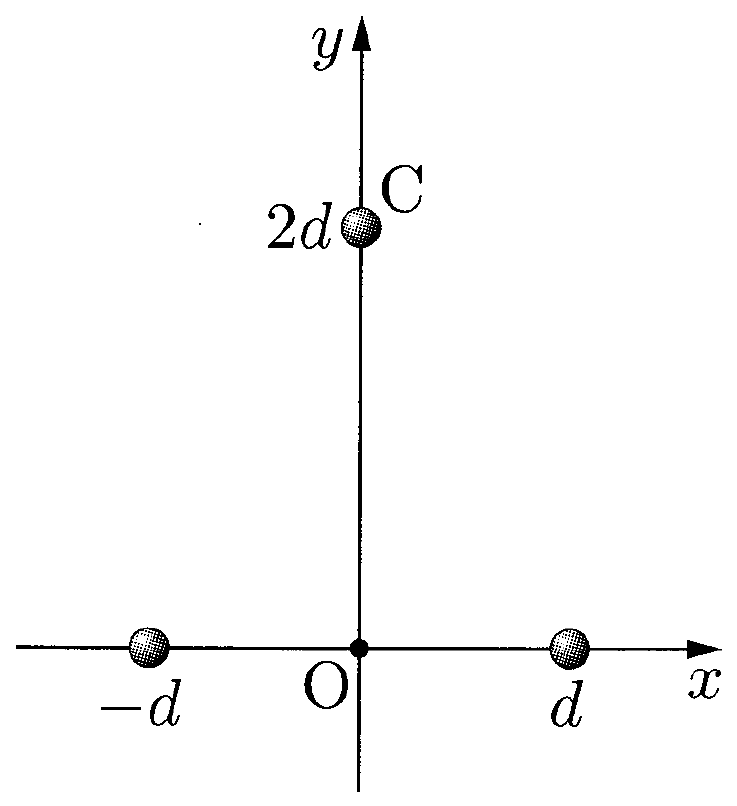
\includegraphics[keepaspectratio,width=52mm]{fig/n24_p37_zu.png}
\end{zuright}

\Mon{電気力線}

\hspace{1zw}絶対値の等しい二つの電荷を次図のように配置した．このとき，この紙面上における電場のおおまかな様子を，電気力線を用いて表せ．ただし，一つの点電荷からはこの平面上において6本の電気力線が出入りしているものとして描け．

\begin{center}
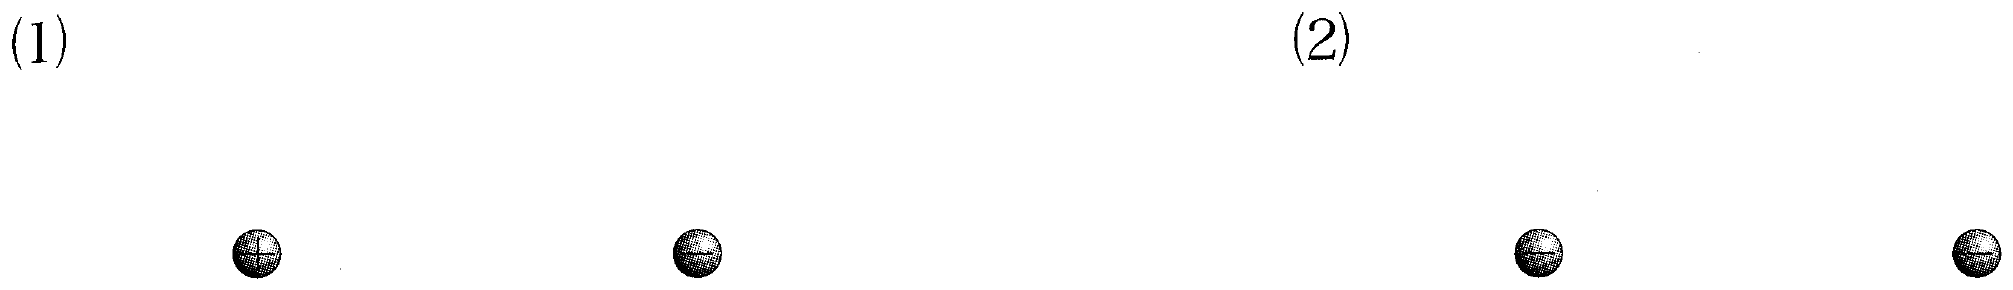
\includegraphics[keepaspectratio,width=142mm]{fig/n24_p38_zu.png}
\end{center}
\vspace{34mm}

\Mon{箔検電器}

\begin{zuright}{34mm}
\hspace{1zw}図のように，ガラスの絶縁びんに金属棒を通し，これに金属箔を取り付けた装置を箔検電器と呼ぶ．最初，箔検電器には電荷がなかった．以下の問に答えよ．
\begin{komon}
\ko{1} 毛皮でこすり，負に帯電したエボナイト棒を金属板に近づけた場合，金属箔がどのようになるか，説明せよ．
\ko{2} (1)の状態で金属板を一度接地し，その接地を外した後でエボナイト棒を遠ざけた．金属箔がどのようになるか，説明せよ．
\end{komon}
\zusep
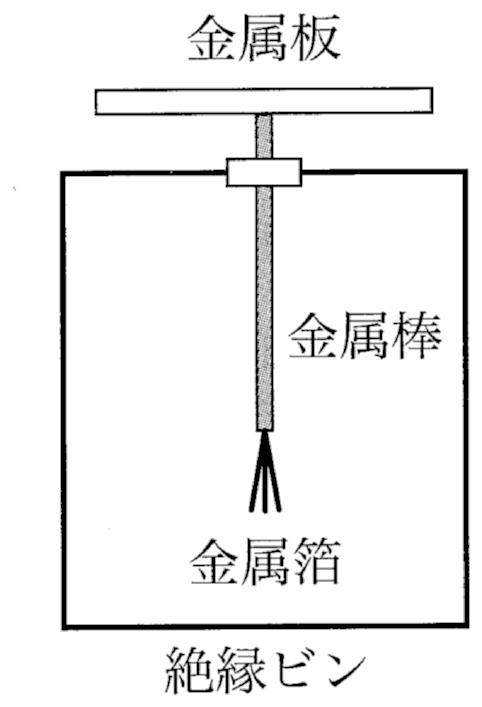
\includegraphics[keepaspectratio,width=34mm]{fig/n24_p39_zu.png}
\end{zuright}

\Mon[\Sitei]{静電誘導}

\begin{zuright}{38mm}
\hspace{1zw}右図のように，負に帯電した帯電棒と箔検電器を用いて次の順に操作を行った．箔検電器の金属板と箔の部分に存在する電荷の分布状態，および箔の開きを各々について図示せよ．
\begin{komon}
\ko{1} 帯電していない箔検電器の金属板に，負に帯電した帯電棒を近づける．
\ko{2} 帯電棒を近づけたまま金属板をアース（接地）する．
\ko{3} 帯電棒を近づけたまま，アースを切る．
\ko{4} 帯電棒を遠ざける．
\end{komon}
\zusep
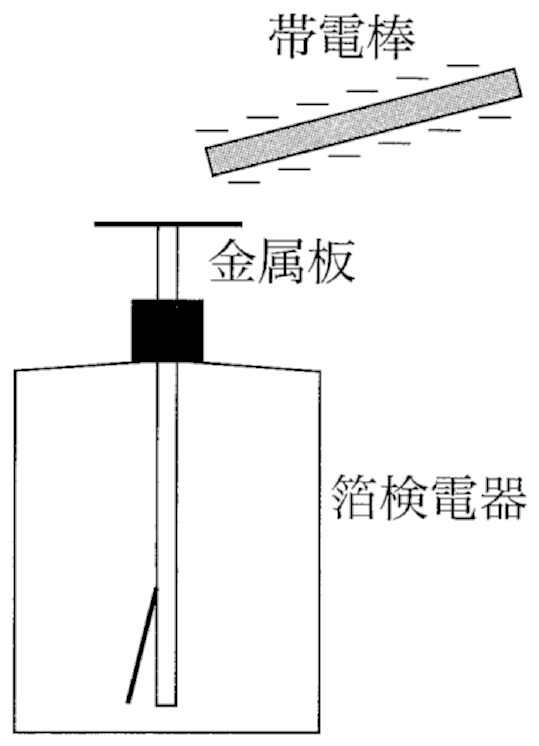
\includegraphics[keepaspectratio,width=38mm]{fig/n24_p40_zu.png}
\end{zuright}

\Mon{電場が物体に対してなす仕事}

\begin{zuright}{62mm}
\hspace{1zw}強さ$E\U{V/m}$の一様電場において，$+q\U{C}$の正電荷を点$\mathrm{A}$から点$\mathrm{C}$まで移動させる（ただし$\overline{\mathrm{AB}}=d\U{m}$である）とき，静電気力のする仕事を仕事の定義に従ってそれぞれ求めよ．
\begin{komon}
\ko{1} $\mathrm{A}$から$\mathrm{C}$へまっすぐ移動させる．
\ko{2} まず$\mathrm{A}$から電気力線に沿って$\mathrm{B}$まで移動させ，続いて$\mathrm{B}$から$\mathrm{C}$までは電気力線に対して垂直に移動させる．
\end{komon}
\zusep
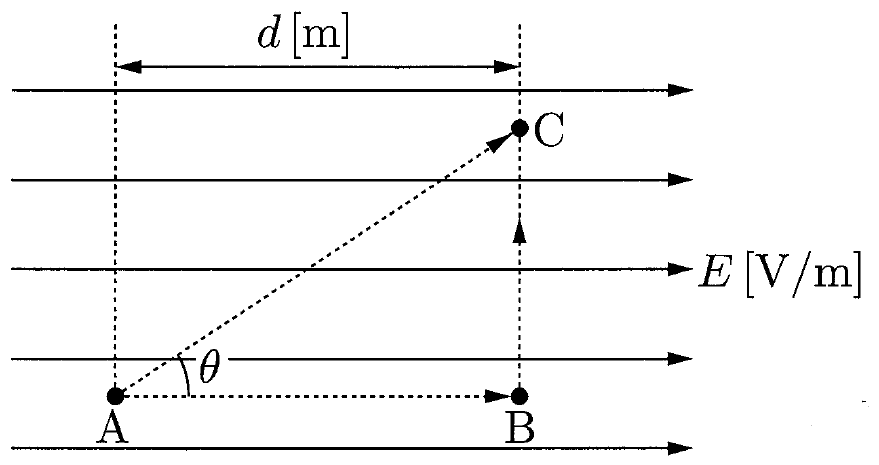
\includegraphics[keepaspectratio,width=62mm]{fig/n24_p41_zu.png}
\end{zuright}

\Mon[\Sitei]{一様電場と電位差}

\begin{zuright}{64mm}
\hspace{1zw}真空中に，厚さが一様な2枚の金属の平行極板$\mathrm{A}$，$\mathrm{B}$と，これらから等距離の位置に金属の薄い平面極板$\mathrm{C}$をそれぞれ平行になるように置く．$\mathrm{A}$，$\mathrm{B}$の間隔は$2d\U{m}$で，各極板の大きさは$d$に比べて十分に大きく，厚さは$d$に比べて十分に小さい．極板$\mathrm{A}$を接地し，電圧$V\U{V}$の二つの電池を図のように接続し，極板$\mathrm{B}$の電位を$-V\U{V}$，極板$\mathrm{C}$の電位を$+V\U{V}$になるようにした．極板$\mathrm{A}$上の点を原点$\mathrm{O}$とし，極板に対して垂直右向きに$x$軸を取るものとして，以下の設問に答えよ．
\zusep
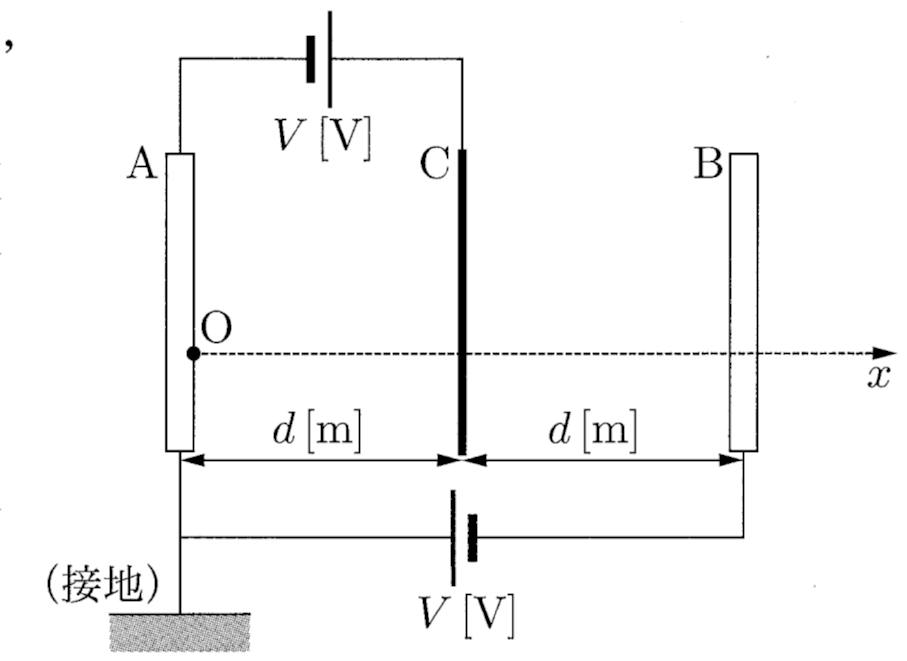
\includegraphics[keepaspectratio,width=64mm]{fig/n24_p42_zu.png}
\end{zuright}
\begin{komon}
\ko{1} 極板$\mathrm{AC}$，$\mathrm{CB}$間に生じる電場の向きおよび大きさを求めよ．
\ko{2} 極板間の任意の点$(0\leqq x\leqq 2d)$における電位$V(x)\U{V}$を求め，グラフを描け．
\end{komon}

\Mon[\Sitei]{点電荷による電場と電位}

\hspace{1zw}図のように$x$軸上の点$\mathrm{O}$，および$x=d\U{m}$の点$\mathrm{A}$にそれぞれ点電荷$+2q\U{C}$，$-q\U{C}$を固定する．クーロンの法則の比例定数を$k\U{N\cdot m^2/C^2}$として，以下の設問に答えよ．ただし$q>0$とする．

\begin{center}
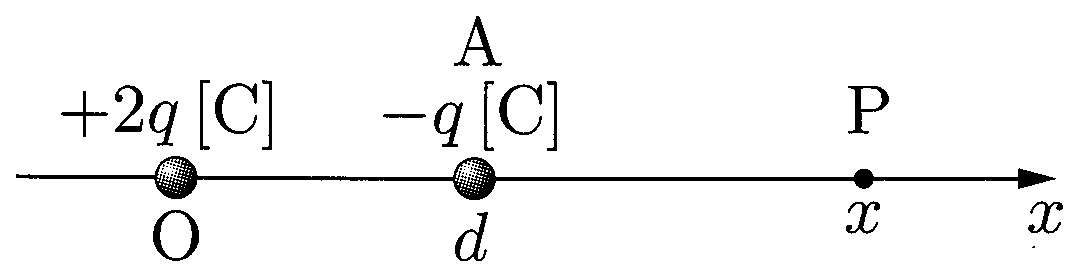
\includegraphics[keepaspectratio,width=92mm]{fig/n24_p43_zu.png}
\end{center}

\begin{komon}
\ko{1} 点$\mathrm{O}$，点$\mathrm{A}$を除く，$x$軸上の任意の点$\mathrm{P}$（座標$x\U{m}$）における電場$E(x)\U{N/C}$を求めよ．ただし，$+x$方向を電場の正の向きとする．
\ko{2} 点$\mathrm{O}$，点$\mathrm{A}$を除く，$x$軸上の任意の点$\mathrm{P}$（座標$x\U{m}$）における電位$V(x)\U{V}$を求めよ．ただし，無限遠方を電位の基準点とする．
\end{komon}

\filbreak
\Rank{C問題}

\Mon{クーロンの法則と力のつり合い}

\begin{zuright}{62mm}
\hspace{1zw}一辺の長さが$2a\U{m}$の立方体の各頂点$(\pm a,\ \pm a,\ \pm a)\U{m}$に，右図のように4個の正電荷$+q\U{C}$と4個の負電荷$-q\U{C}$を置き，正の電荷$+Q\U{C}$を持つ質量$m\U{kg}$の質点$\mathrm{P}$を立方体の中心$\mathrm{O}$に置いたところ，$\mathrm{P}$に作用するクーロン力と重力とがつり合った．
\par\hspace{1zw}$\mathrm{P}$を立方体の上面の中心$\mathrm{A}$に置くとき，$\mathrm{P}$に作用するクーロン力と重力の合力はどちらを向いているか．またその合力の大きさは，$\mathrm{P}$に作用する重力の大きさの何倍か．
\zusep
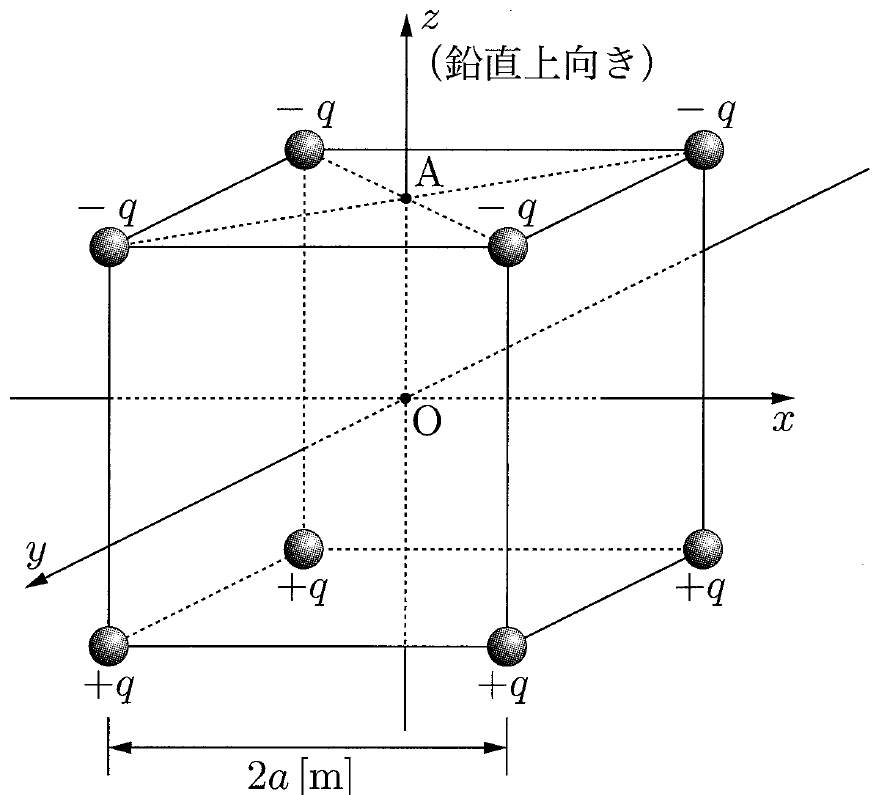
\includegraphics[keepaspectratio,width=62mm]{fig/n24_p44_zu.png}
\end{zuright}

\Mon{等電位線と仕事}

\begin{zuright}{58mm}
\hspace{1zw}右図のような等電位線をもつ電場中を，図中の矢印の向きに沿って$\mathrm{A}\rightarrow\mathrm{B}\rightarrow\mathrm{C}\rightarrow\mathrm{D}\rightarrow\mathrm{E}\rightarrow\mathrm{A}$の順に$+5\U{C}$の正電荷をゆっくりと移動させるときについて考える．
\begin{komon}
\ko{1} $\mathrm{AB}$，$\mathrm{BC}$，$\mathrm{CD}$，$\mathrm{DE}$，$\mathrm{EA}$の各区間で，外力がした仕事をそれぞれ求めよ．
\ko{2} (1)で求めた仕事の総和はいくらか．
\ko{3} 図から判断して，点$\mathrm{A}$と点$\mathrm{D}$とではどちらが電場が強いか．理由を付けて答えよ．
\end{komon}
\zusep
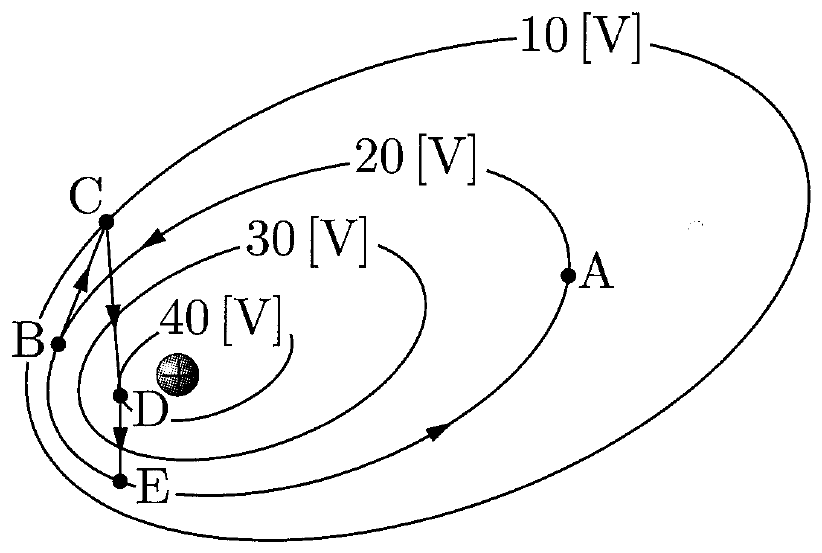
\includegraphics[keepaspectratio,width=58mm]{fig/n24_p45_zu.png}
\end{zuright}

\Mon{電場と仕事}

\begin{zuright}{50mm}
\hspace{1zw}右図に示したアからクは，点$\mathrm{O}$を中心とする半径$r\U{m}$の円周を8等分する点である．この空間に，一様な強さの電場を直径アオに対して平行に加える．次に電荷$+q\U{C}$を持つ小球を点$\mathrm{O}$に固定した．クーロンの法則の比例定数を$k\U{N\cdot m^2/C^2}$として以下の設問に答えよ．
\begin{komon}
\ko{1} 電荷$-q\U{C}$を持つ第2の小球$\mathrm{M}$を点アの位置に置いたところ，$\mathrm{M}$は静止したままであった．一様な電場の強さおよび向きを求めよ．
\ko{2} 次にこの小球$\mathrm{M}$を点アの位置から円周上をア$\rightarrow$イ$\rightarrow$ウ$\rightarrow$エの順に，点エの位置まで外力を加えてゆっくりと動かした．この移動の間に外力が$\mathrm{M}$にした仕事$W\U{J}$を求めよ．
\end{komon}
\zusep
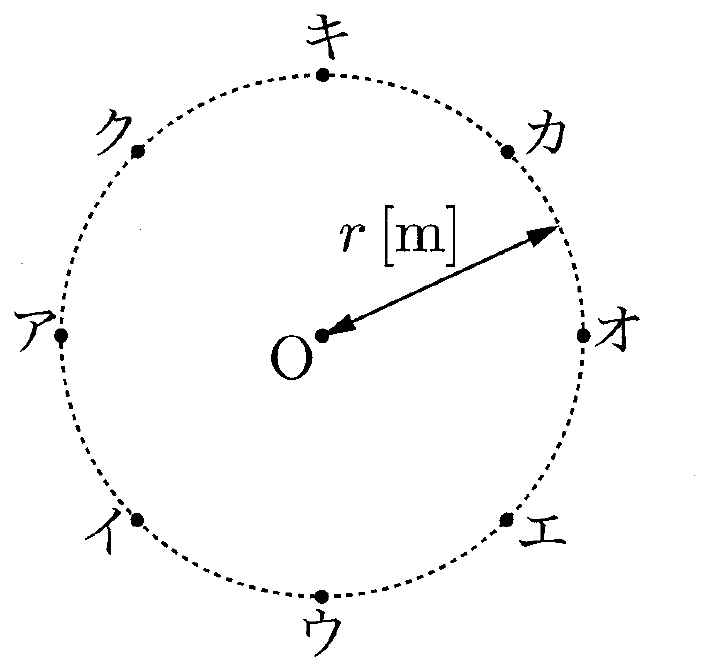
\includegraphics[keepaspectratio,width=50mm]{fig/n24_p46_zu.png}
\end{zuright}

\newpage

%%%%%%%%%%%%%%%%%%%%  解答  %%%%%%%%%%%%%%%%%%%%
\KaiTitle{第24回　静電気力・電場・電位}
\setlength{\columnseprule}{0.4pt}
\begin{multicols}{2}
\raggedcolumns

\Rank{A問題}
\MonN{34}{基本公式の確認}\par\nopagebreak
\begin{sisin}
(1)〜(3) クーロンの法則$f=k\dfrac{|q_1q_2|}{r^2}\U{N}$を利用して考える．{\gtfamily 大きさと向きとを分けて}考えるとよい．まずは電荷$q_1$, $q_2\U{C}$の絶対値を取って式に代入して，クーロン力の大きさを求める．続いて，二つの電荷が同符号か異符号かを考えて力の作用する向きを決定する．多少まわりくどいが，この方法の方が確実である．

(4)〜(6) 一様電場の場合と点電荷の場合それぞれについて，電位と電場の関係式および扱い方の違いを比較し，混同しないようにせよ．分かりにくい場合には，電位と座標の関係のグラフを図示しながら考えていくとよい．点電荷の作る電位の式$V(r)=k\dfrac{q}{r}$を利用する際には，$q$には{\gtfamily 符号付きで}電気量を代入せよ．
\end{sisin}
\KaiHead
\begin{komon}
\ko{1} 二つの電荷は異符号ゆえ引力を及ぼし合う．その作用しあう力の大きさは，
       \[\begin{aligned}
         f&=k\frac{|q_1q_2|}{r^2}=9.0\times 10^9\cdot\frac{1.0\cdot 4.0}{100^2}\\
          &=3.6\times 10^6\U{N}\Ans
       \end{aligned}\]
\ko{2} この点電荷は正電荷であるから，点電荷は外向きの電場を作る．$\mathrm{A}$点における電場の強さは，
       \[\begin{aligned}
         E&=k\frac{|q|}{r^2}=9.0\times 10^9\cdot\frac{7.0\times 10^{-8}}{0.30^2}\\
          &=7.0\times 10^3\U{N/C}\Ans
       \end{aligned}\]
       また，向きは
       \[\text{点電荷から点$\mathrm{A}$へ向かう向き}\Ans\]
\ko{3} この電荷は負電荷であるから，電場とは逆向きに力を受けている．よって，電場の向きは
       \[\text{左向き}\Ans\]
       また，電場の強さを$E\U{N/C}$とすると，受ける力の大きさと電荷，電場の強さとの間の関係式は
       \[F=|q|E\]
       であるからこれを解いて，
       \[E=\frac{8.0\times 10^{-5}}{4.0\times 10^{-8}}=2.0\times 10^3\U{N/C}\Ans\]
\ko{4} 一様電場であるから，電位差は
       \[\Delta V=E\cdot d=3.0\cdot 1.5=4.5\U{V}\Ans\]
\ko{5} 点電荷であるから，電位は
% 誤植訂正（2026-09-23）：原本の解答は $V=k\dfrac{q}{Q}$ と書かれていたが，
%   代入している値（2.0）は距離なので $V=k\dfrac{q}{r}$ が正しい．
       \[\begin{aligned}
         V&=k\frac{q}{r}=9.0\times 10^9\cdot\frac{-5.6\times 10^{-6}}{2.0}\\
          &\fallingdotseq -2.5\times 10^4\U{V}\Ans
       \end{aligned}\]
\ko{6} ゆっくりと動かしているので，運動エネルギーは$0$のまま変化しない．ゆえに，外力のした仕事はすべて物体の位置エネルギーの増加に利用されている．よって$\mathrm{AB}$間の電位差（$\mathrm{B}$の方が高い場合を正とする）を$\Delta V\U{V}$とすると，
       \[8.0=(+0.25)\cdot\Delta V\]
       であるから，
       \[\Delta V=32\U{V}\]
       であり，$\Delta V>0$であるから$\mathrm{B}$の方が電位が高い．\Ans
\end{komon}

\Rank{B問題}
\MonN{35}{クーロンの法則}\par\nopagebreak
\begin{sisin}
クーロンの法則は，力の大きさと向きとを分けて考える．電荷の大きさについては，電荷について絶対値を取って代入して力の大きさを求める式である
\[f=k\frac{|q_1q_2|}{r^2}\U{N}\]
を利用して求め，また電荷の正負は及ぼし合う力が引力，斥力のどちらであるかを元にして考える．
\end{sisin}
\KaiHead
$\mathrm{A}$, $\mathrm{B}$, $\mathrm{C}$の電気量の大きさ（絶対値）をそれぞれ$q_{\mathrm{A}}$, $q_{\mathrm{B}}$, $q_{\mathrm{C}}\U{C}$とおく．まず，$\mathrm{B}$は負電荷であるとあるので，その電気量は$-q_{\mathrm{B}}\U{C}$とおける．

$\mathrm{A}$, $\mathrm{B}$は互いに引力を及ぼし合うので二つの電荷は異符号である．よって$\mathrm{A}$は正電荷であるから，$\mathrm{A}$の電気量は$+q_{\mathrm{A}}\U{C}$と決められる．また，$\mathrm{B}$と$\mathrm{C}$は互いに斥力を及ぼし合うので二つの電荷は同符号である．よって$\mathrm{C}$は負電荷であるから，$\mathrm{C}$の電気量は$-q_{\mathrm{C}}\U{C}$と決められる．

次に，$\mathrm{AB}$間，$\mathrm{BC}$間，$\mathrm{CA}$間で及ぼし合う力の大きさを書き下すと，
\[f_1=k\frac{q_{\mathrm{A}}q_{\mathrm{B}}}{r^2},\quad f_2=k\frac{q_{\mathrm{B}}q_{\mathrm{C}}}{r^2},\quad f_3=k\frac{q_{\mathrm{C}}q_{\mathrm{A}}}{r^2}\]
であるから，これら3式を解いて，各電荷の電気量の絶対値はそれぞれ
\[q_{\mathrm{A}}q_{\mathrm{B}}q_{\mathrm{C}}=r^3\sqrt{\frac{f_1f_2f_3}{k^3}}\]
より，
\[q_{\mathrm{A}}=r\sqrt{\frac{f_1f_3}{kf_2}},\quad q_{\mathrm{B}}=r\sqrt{\frac{f_1f_2}{kf_3}}\U{C}\]
\[q_{\mathrm{C}}=r\sqrt{\frac{f_2f_3}{kf_1}}\U{C}\]
である．以上より，$\mathrm{A}$, $\mathrm{B}$, $\mathrm{C}$の電荷はこれらに符号をつけて，
\[\left\{\begin{aligned}
 &\mathrm{A}\text{の電荷}:+q_{\mathrm{A}}=+r\sqrt{\frac{f_1f_3}{kf_2}}\U{C}\\
 &\mathrm{B}\text{の電荷}:-q_{\mathrm{B}}=-r\sqrt{\frac{f_1f_2}{kf_3}}\U{C}\\
 &\mathrm{C}\text{の電荷}:-q_{\mathrm{C}}=-r\sqrt{\frac{f_2f_3}{kf_1}}\U{C}
\end{aligned}\right.\Ans\]

\MonN{36}{クーロンの法則と力のつり合い}\par\nopagebreak
\begin{sisin}
まずは物体に作用する力を書き出していこう．$\MARU{1}$場の力$\rightarrow$重力，クーロン力の二つ（クーロン力とは電場という場から受ける力であるから場の力に分類される），$\MARU{2}$接触力$\rightarrow$張力，$\MARU{3}$作用・反作用，の順番で力を押さえる．

クーロン力の大きさを求める際の，二物体間の距離に注意．本問の図の場合には$l\sin\theta\U{m}$ではなく$2l\sin\theta\U{m}$である．
\end{sisin}
\KaiHead
\begin{komon}
\ko{1} 物体には大きさ$mg\U{N}$の重力，大きさ$T\U{N}$の張力，およびクーロン力の三つの力が作用するが，このとき二つの電荷が異符号の場合にはクーロン力は引力となり，次図のように力が作用するため，この小球は力がつり合わなくなってしまう．
       \begin{center}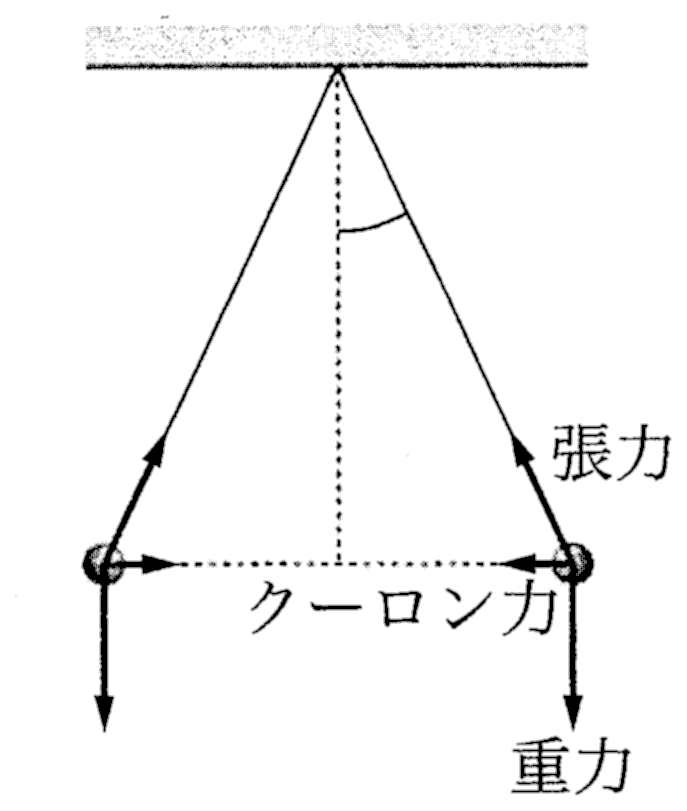
\includegraphics[keepaspectratio,width=52mm]{fig/n24_a36_zu2.png}\end{center}
       よって，二つの電荷は互いに同符号である．\Ans
\ko{2} (1)より小球の持つ電荷は互いに同符号であり，斥力を及ぼし合うので，力の作用図は次のようになる．
       \begin{center}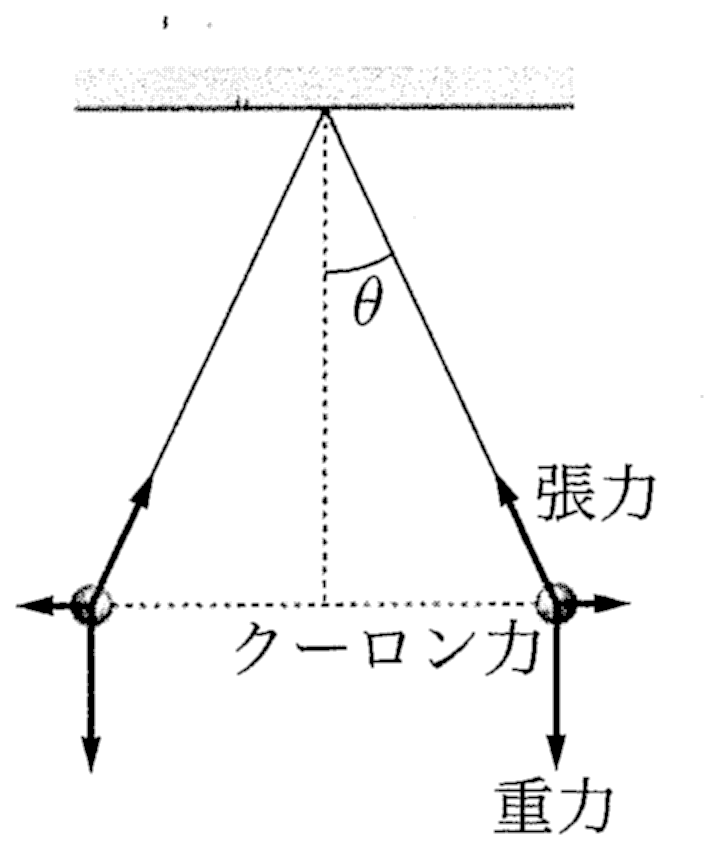
\includegraphics[keepaspectratio,width=52mm]{fig/n24_a36_zu1.png}\end{center}
       この二つの電荷が及ぼし合うクーロン力は，電気量の絶対値がいずれも$q\U{C}$，2点間の距離が$2l\sin\theta\U{m}$であることに注意すると$k\dfrac{q^2}{(2l\sin\theta)^2}\U{N}$である．この小球について力のつり合いの式を立てると，
       \[\left\{\begin{aligned}
        &\text{鉛直方向}:T\cos\theta=mg\\
        &\text{水平方向}:T\sin\theta=k\frac{q^2}{(2l\sin\theta)^2}
       \end{aligned}\right.\Ans\]
\ko{3} (2)より$T$を消去して解き，（大きさゆえ）$q>0$として平方根を取ると，
       \[q=2l\sin\theta\sqrt{\frac{mg}{k}\tan\theta}\U{C}\Ans\]
\end{komon}

\MonN[\Sitei]{37}{クーロン力と電場}\par\nopagebreak
\begin{sisin}
電場はベクトルで表される量（$\overrightarrow{E}$と書かれる）であり，向きと大きさを持つものである（大きさは「電場の強さ」と呼ばれる）．よって，二つの点電荷が作る電場を合成する場合には，大きさを単純和するのではなく，{\gtfamily 向きを図示してベクトル合成しなければならない}．

$\mathrm{A}$点の電荷が$\mathrm{C}$点に作る電場を考える際には，{\gtfamily $\mathrm{AC}$間に直線を引き}，これを補助線として利用せよ．$\mathrm{C}$点に作られる電場はこの直線方向であり，また$E=k\dfrac{q}{r^2}$の分母に代入する値は{\gtfamily $\mathrm{AC}$間の直線距離}である．

電場の向きは，その点に$+1\U{C}$の単位正電荷を置いて考えれば簡単に判断できる．$+1\U{C}$の単位正電荷が受ける力の向きが電場の向きである．
\end{sisin}
\KaiHead
\begin{komon}
\ko{1} まず$\mathrm{A}$点の$+q\U{C}$の点電荷が$\mathrm{C}$点に作る電場を考える．$\mathrm{A}$点の点電荷は正電荷ゆえ外向きに電場を作るので，$\mathrm{C}$点に対しては$\overrightarrow{\mathrm{AC}}$向きの電場を作る．また$\overline{\mathrm{AC}}=\sqrt{5}\,d\U{m}$であるから，$\mathrm{A}$点の点電荷が$\mathrm{C}$点に作る電場の強さ（大きさ）は，
       \[E_{\mathrm{A}}=k\frac{q}{\left(\sqrt{5}\,d\right)^2}\U{N/C}\]
       である．
       \begin{center}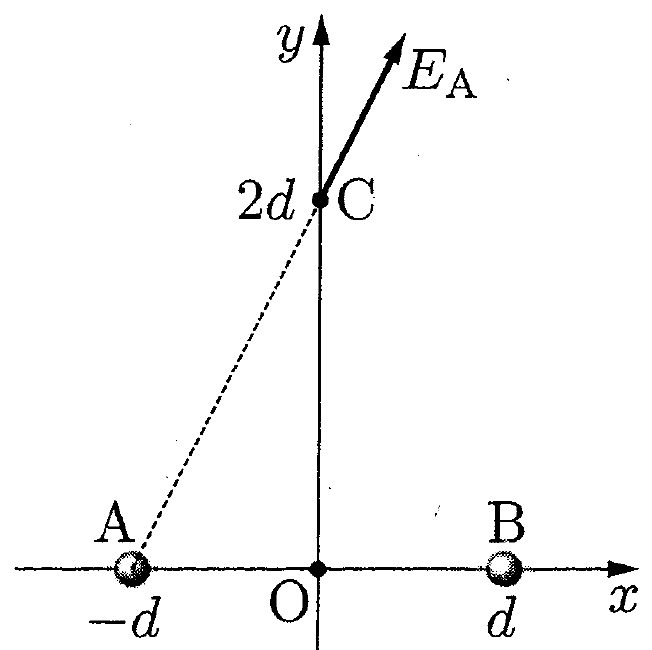
\includegraphics[keepaspectratio,width=46mm]{fig/n24_a37_ea.png}\end{center}
       次に，$\mathrm{B}$点の$-q\U{C}$の点電荷が$\mathrm{C}$点に作る電場を考える．$\mathrm{B}$点の点電荷は負電荷ゆえ内向きに電場を作るので，$\mathrm{C}$点に対しては$\overrightarrow{\mathrm{CB}}$向きの電場を作る．また$\overline{\mathrm{BC}}=\sqrt{5}\,d\U{m}$であるから，$\mathrm{B}$点の点電荷が$\mathrm{C}$点に作る電場の強さは，
       \[E_{\mathrm{B}}=k\frac{q}{\left(\sqrt{5}\,d\right)^2}\U{N/C}\]
       である．
       \begin{center}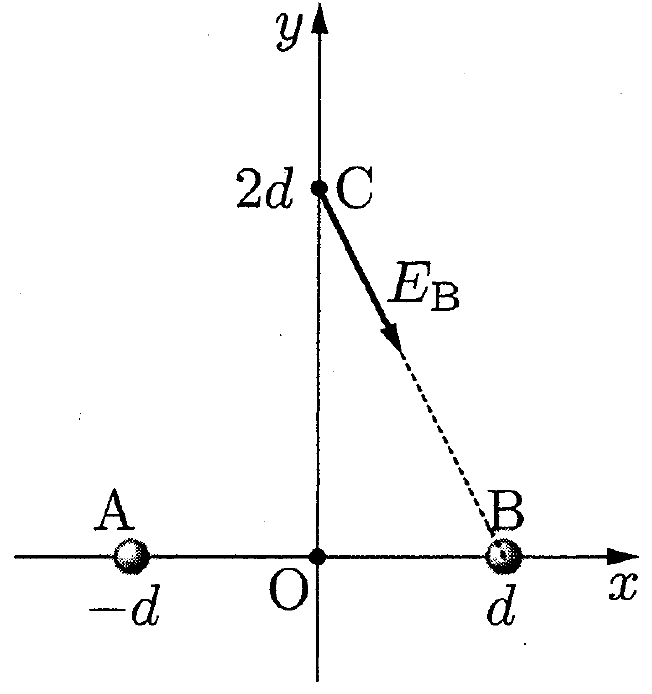
\includegraphics[keepaspectratio,width=46mm]{fig/n24_a37_eb.png}\end{center}
       $\mathrm{C}$点に作られている電場は，この二つの電場ベクトルのベクトル合成である．$\angle\mathrm{AOC}=\theta$とし，二つの電場ベクトルの大きさが同じであることに注意してベクトル和を取ると，合成電場は$+x$方向を向いている．\Ans
       \begin{center}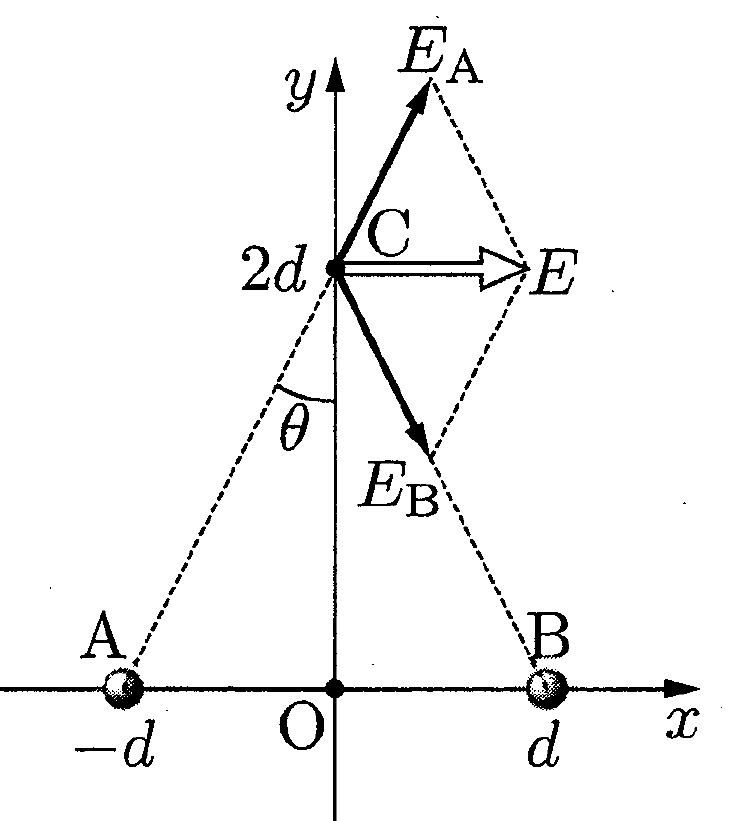
\includegraphics[keepaspectratio,width=52mm]{fig/n24_a37_sum.png}\end{center}
       また，その大きさは，
       \[E=E_{\mathrm{A}}\times 2\sin\theta\]
       である．図より$\sin\theta=\dfrac{1}{\sqrt{5}}$であるから，
       \[E=\frac{2kq}{5\sqrt{5}\,d^2}\U{N/C}\Ans\]
\ko{2} 配置する点電荷$-q\U{C}$は負電荷であるから，その点の電場とは逆向きに力を受ける．よって，この点電荷が受ける力の向きは$-x$方向である．\Ans\par
       またその大きさは，
       \[F=|-q|E=\frac{2kq^2}{5\sqrt{5}\,d^2}\U{N}\Ans\]
\end{komon}

\MonN{38}{電気力線}\par\nopagebreak
\begin{sisin}
電気力線とは，電場を滑らかな曲線群で表したものであり，厳密に電気力線を描くためにはまず前問までと同様にして各点ごとの電場の強さを求め，電場の強さと電気力線の密度を対応づけ，また向きを合わせて作図していく必要がある．しかし，電気力線は正電荷から発生し，負電荷で消滅する（もしくは無限遠方で出入りする）こと，また電気力線は途中で交わったり枝分かれしたりしないことを考慮すれば，電荷の周辺の電気力線の様子をおおまかには把握でき，これによって作られる電場のおおまかな様子を手っ取り早く知ることができる．
\end{sisin}
\KaiHead
\begin{komon}
\ko{1} 左の正電荷から湧き出した電気力線が右の負電荷に吸い込まれるので，次図のようになる．
       \begin{center}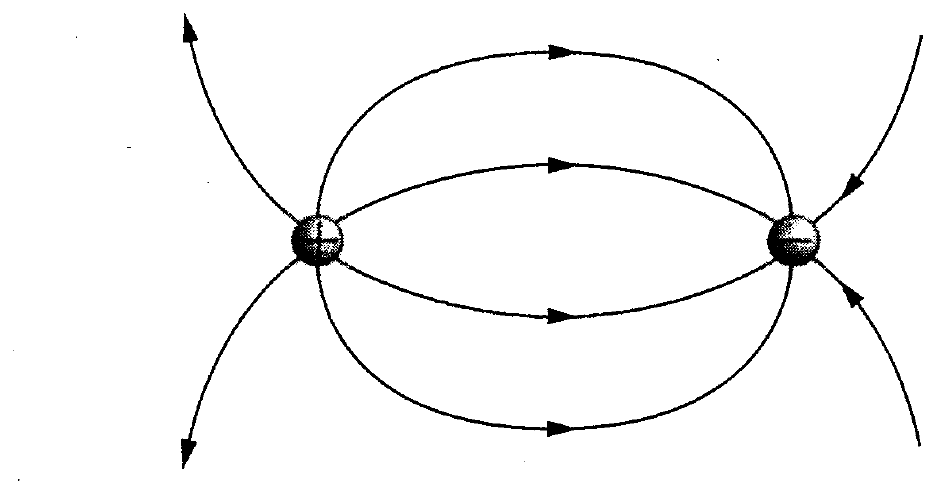
\includegraphics[keepaspectratio,width=66mm]{fig/n24_a38_zu1.png}\end{center}
       \hspace*{\fill}\Ans
\ko{2} 二つとも負電荷であるから，無限遠方から電気力線を吸い込む．中心付近では上下から流れ込んだ電気力線が左右に分かれて負電荷に吸い込まれる．
       \begin{center}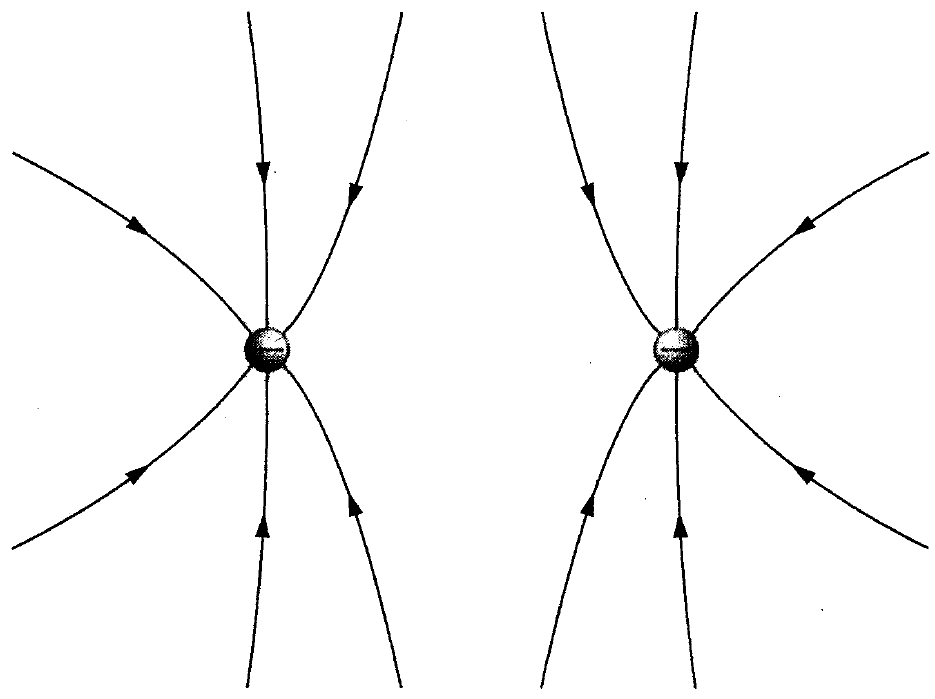
\includegraphics[keepaspectratio,width=66mm]{fig/n24_a38_zu2.png}\end{center}
       \hspace*{\fill}\Ans
\end{komon}

\MonN{39}{箔検電器}\par\nopagebreak
% 原本の【例題4】を練習へ降ろしたもの（`saihen/電磁気_例題配分.md`）。
%   原本には指針しか無いので，解答は新たに書き起こした。図は旧㉙[6]の解答図を流用している。
\begin{sisin}
電荷の分布の様子を$+$，$-$によって図示しながら考えるとよい．

実際に物体間を移動するのは{\gtfamily 電子}であり，正電荷を持つ陽イオンは移動しない．「正に帯電した」とは電子が不足したという意味であることに注意せよ．
\end{sisin}
\KaiHead
\begin{komon}
\ko{1} 負に帯電したエボナイト棒を近づけると，金属板の自由電子が棒の負電荷から反発を受けて箔の部分へ移動する．その結果，金属板は陽イオン過剰となって正に，箔は電子過剰となって負に帯電する．よって{\gtfamily 箔は負電荷同士の反発によって開く}．\Ans
       \begin{center}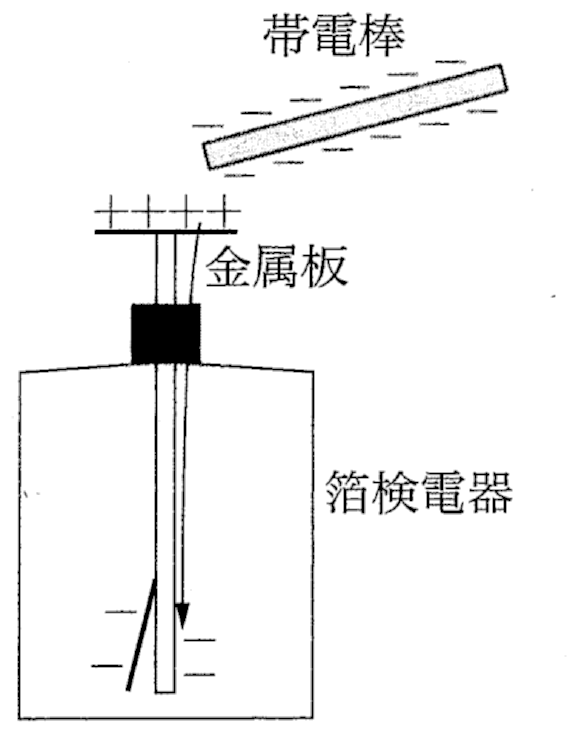
\includegraphics[keepaspectratio,width=40mm]{fig/n24_a40_zu1.png}\end{center}
\ko{2} 金属板を接地すると，箔へ逃げていた自由電子はさらに広い地球へと逃げていくので，箔は帯電しなくなり閉じる．この状態で接地を外すと自由電子の出入りができなくなるので，箔検電器全体としては{\gtfamily 電子が不足したまま}である．

       ここでエボナイト棒を遠ざけると，金属板に引き寄せられていた理由が無くなるので，不足した電子による正電荷は箔検電器全体に拡散する．よって金属板・箔ともに正に帯電し，{\gtfamily 箔は正電荷同士の反発によって再び開く}．\Ans
       \begin{center}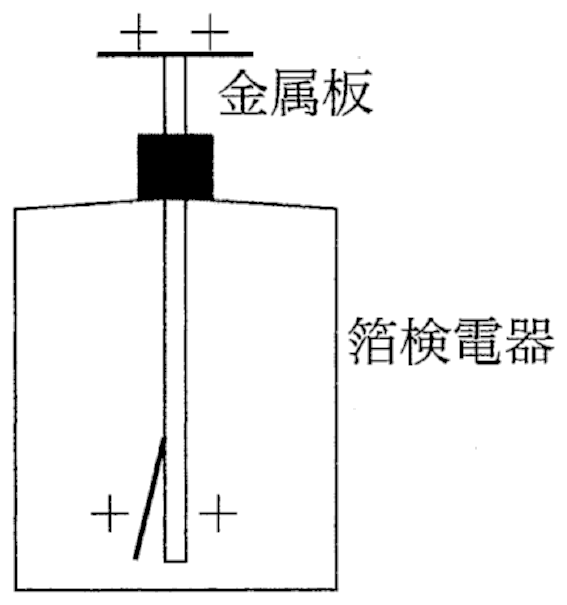
\includegraphics[keepaspectratio,width=40mm]{fig/n24_a40_zu4.png}\end{center}
\end{komon}

\MonN[\Sitei]{40}{静電誘導}\par\nopagebreak
\begin{sisin}
一つずつの操作でどのように電荷が移動するのかを，順番に図示していくことで考えていこう．「$\MARU{1}$同種の電荷同士は反発しあい，可能な限り拡散しようとする．$\MARU{2}$異種の電荷同士は引き合い，なるべく近づこうとする．」の二つの知識を利用せよ．

アース（地球）は非常に大量の正電荷・負電荷を持っているために，正電荷・負電荷が自由に出入りすることができる．アース自体が非常に大きな体積を持っていることに着目すると分かりやすい．

実際に物体間を移動するのは電子であり，正電荷を持つ陽イオンは移動せず，帯電は電子の過不足によって起こることに注意せよ．
\end{sisin}
\KaiHead
\begin{komon}
\ko{1} 帯電棒を近づけることにより，金属板の自由電子が反発して箔の部分に移動し，金属板は陽イオン過剰となって正に，そして箔は電子過剰となって負に帯電する．よって箔検電器の金属板と箔の部分に存在する電荷の分布状態は次図の通りとなり，箔は負電荷同士の反発によって開く．\Ans
       \begin{center}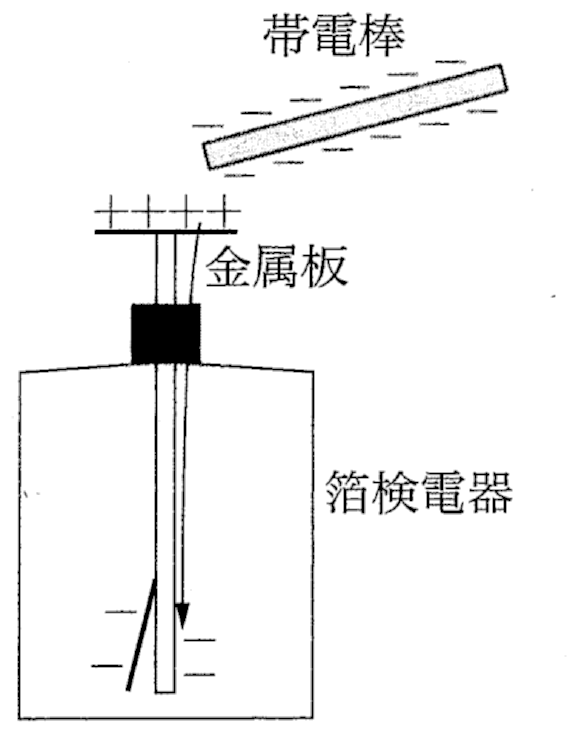
\includegraphics[keepaspectratio,width=40mm]{fig/n24_a40_zu1.png}\end{center}
\ko{2} この状態で金属板をアースすると，金属板から箔検電器の方に逃げていた自由電子がアースの方へと逃げていく（アースへ逃げれば地球全体に拡散することができるため）．
       \begin{center}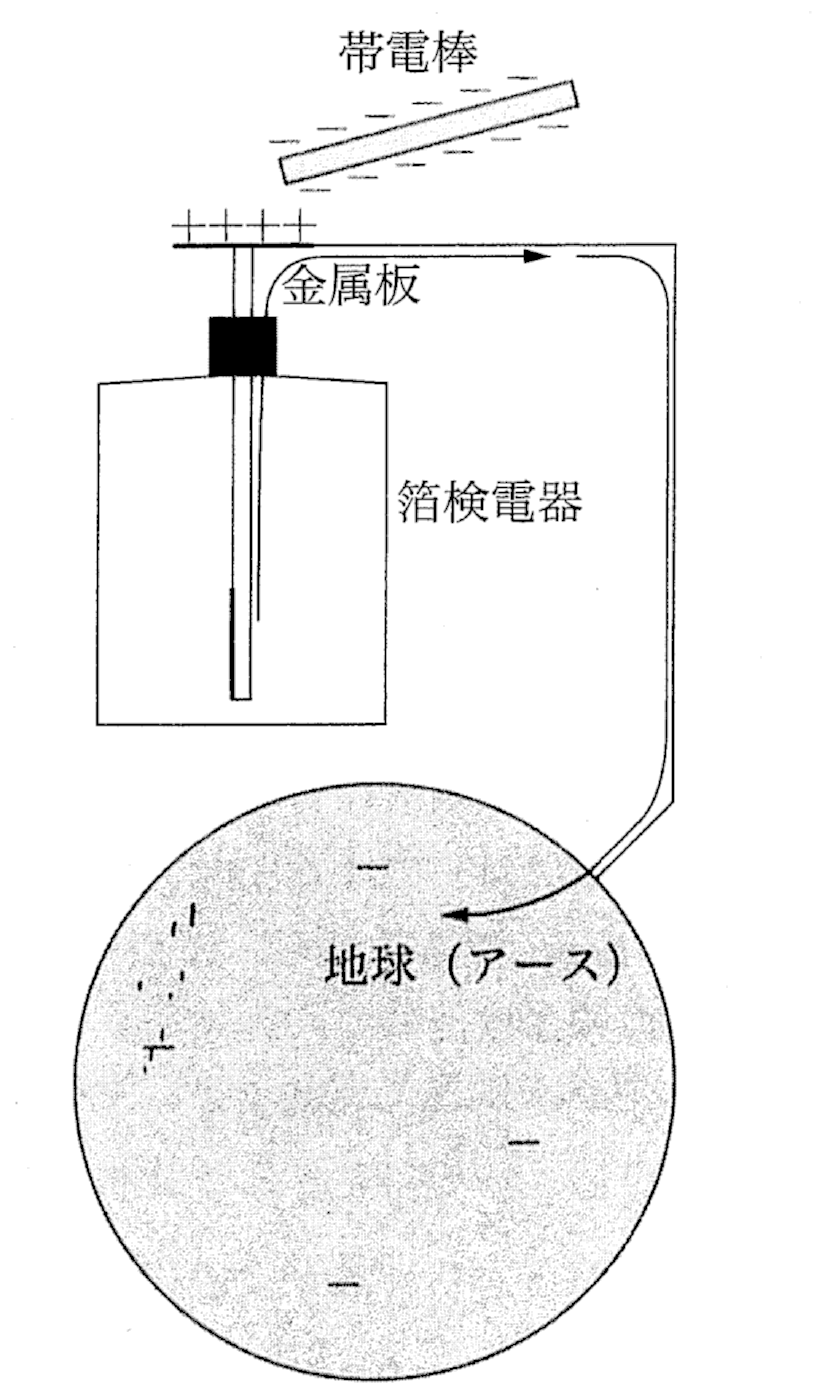
\includegraphics[keepaspectratio,width=58mm]{fig/n24_a40_zu2.png}\end{center}
       よって，帯電棒の負電荷の反発を受けた電子は箔ではなくアースの方へと逃げるため，金属板は取り残された陽イオンによって正に帯電．また，金属箔は帯電しないので，箔は開かない．\Ans
\ko{3} 帯電棒を近づけたままの状態でアースを切り離しても自由電子の移動はなく，変化は起こらない．よって金属板と箔の部分に存在する電荷の分布状態は(2)と変わらず，箔は閉じたままである．\Ans
       \begin{center}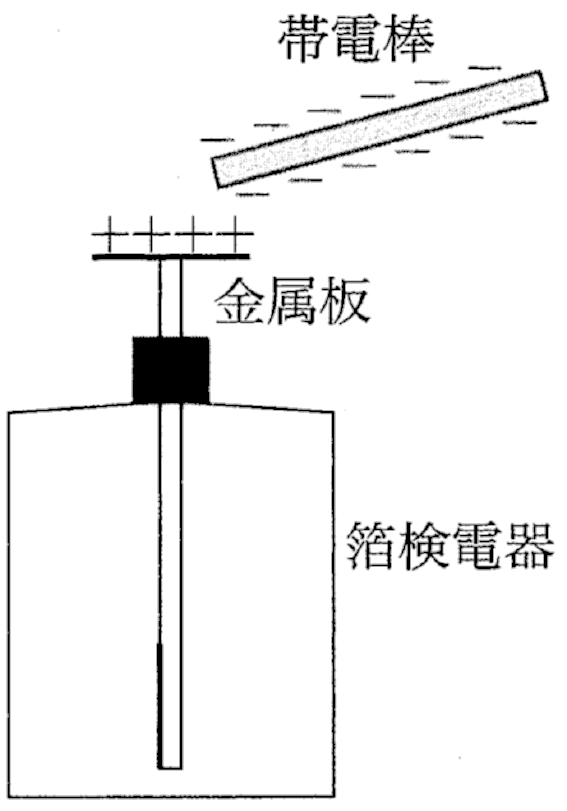
\includegraphics[keepaspectratio,width=40mm]{fig/n24_a40_zu3.png}\end{center}
\ko{4} 帯電棒を遠ざけると，箔の部分の自由電子が陽イオン過剰の金属板側に引き寄せられ，金属板の正電荷が一部打ち消されると同時に箔が陽イオン過剰となり正に帯電する．よって金属板と箔の部分に存在する電荷はいずれも正電荷であり，箔はこの正電荷同士の反発によって開く．\Ans
       \begin{center}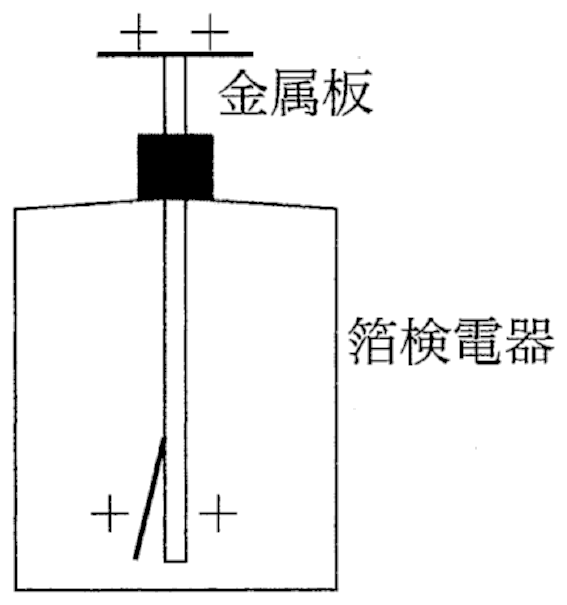
\includegraphics[keepaspectratio,width=40mm]{fig/n24_a40_zu4.png}\end{center}
\end{komon}

\MonN{41}{電場が物体に対してなす仕事}\par\nopagebreak
\begin{sisin}
電場が物体に対してなす仕事は，物体の位置エネルギー変化を元にして計算していくことも可能であるが，本問ではそれを仕事の定義に従って計算してみようという問題である．物体に対して作用する力を図示して，$W=fs\cos\theta$を適用して求めていこう．
\end{sisin}
\KaiHead
一様な電場であるからどの点においても物体が受ける力は同じになる．（正電荷であるから）$\overrightarrow{\mathrm{AB}}$の向きと同じ向きに力を受け，その大きさは$qE\U{N}$である．
\begin{komon}
\ko{1} $\mathrm{A}$から$\mathrm{C}$までまっすぐ移動させるとき，力の作用する方向（$\overrightarrow{\mathrm{AB}}$の向き）と物体の移動方向（$\overrightarrow{\mathrm{AC}}$の向き）とのなす角は$\theta$である．また，$\overline{\mathrm{AC}}=\dfrac{d}{\cos\theta}\U{m}$であるから，
       \[W_1=qE\cdot\overline{\mathrm{AC}}\cdot\cos\theta=qEd\U{J}\Ans\]
\ko{2} まず，$\mathrm{A}$から$\mathrm{B}$まで電気力線に沿って移動させるときには，力の作用する方向（$\overrightarrow{\mathrm{AB}}$の向き）と物体の移動方向（$\overrightarrow{\mathrm{AB}}$の向き）とのなす角は$0^\circ$であるから，この間に静電気力のする仕事は，
       \[W_2=qE\cdot d\cdot\cos 0^\circ=qEd\U{J}\]
       また，$\mathrm{B}$から$\mathrm{C}$まで電気力線に対して垂直に移動させるときには，力の作用する方向（$\overrightarrow{\mathrm{AB}}$の向き）と物体の移動方向（$\overrightarrow{\mathrm{BC}}$の向き）とのなす角は$90^\circ$であるから，この間に静電気力のする仕事は，
       \[W_3=qE\cdot\overline{\mathrm{BC}}\cdot\cos 90^\circ=0\U{J}\]
       である．以上より，静電気力のなす仕事の総和は，
       \[W_2+W_3=qEd\U{J}\Ans\]
\end{komon}
\begin{bsHosoku}{参考}
本問の結果は，$\mathrm{A}$から$\mathrm{C}$点までの移動において，$\mathrm{A}\rightarrow\mathrm{C}$の直接移動でも，または$\mathrm{B}$点を経由して$\mathrm{C}$点へ移動する方法でも，静電気力のする仕事は同じになることを示している．本問では二つの経路のみについて議論したが，実際には$\mathrm{A}$点から$\mathrm{C}$点まで移動させる場合に静電気力がする仕事は，どのような経路をたどって$\mathrm{C}$点に到達する場合であっても必ず同じ値（$qEd\U{J}$）になる．このように，その力のする仕事が物体の最初と最後の位置のみで決まり，途中の経路によらないような力のことを{\gtfamily 保存力}といい，静電気力（クーロン力）の他に，重力，バネの弾性力，万有引力がこの保存力に分類される力である．

また，このような保存力のする仕事$W$は，その保存力に基づく位置エネルギーの変化$\Delta U$と，$\Delta U=-W$の関係を満たす．例えば本問の場合，$\mathrm{A}\rightarrow\mathrm{C}$へ移動したときの電位の変化は$\Delta V=-Ed\U{V}$（図より$\mathrm{C}$の方が低電位なので，$\mathrm{A}\rightarrow\mathrm{C}$の移動による電位の変化はマイナス）であるから，その位置エネルギー変化は
\[\Delta U=(+q)\cdot\Delta V=-qEd\U{J}\]
となり，確かに$\Delta U=-W$の関係が満たされていることが分かる．
\end{bsHosoku}

\MonN[\Sitei]{42}{一様電場と電位差}\par\nopagebreak
\begin{sisin}
本問のような平行極板間には一様な電場が作られるため，極板間の電場の強さは電位差を単純に距離で割り算して，$E=\dfrac{V}{d}\U{V/m}$として求められる．またその向きは，{\gtfamily 電位の高い極板から低い極板に向かって}になる．

また電場が一様な場合には，電位の変化，すなわち(2)のグラフの傾きが一定になる．本問の場合は$\mathrm{A}$, $\mathrm{C}$, $\mathrm{B}$の各極板での電位は明らかであるから，あとはその間を直線で結べば$V(x)\U{V}$のグラフが得られる．

本問のように接地されている極板がある場合には，これを電位の基準点（$0\U{V}$である点）とせよ．

なお，電場の単位は$\U{V/m}$でも$\U{N/C}$でもどちらでもよい（いずれもMKSA単位系で表すと全く同一の単位になる）．
\end{sisin}
\KaiHead
\begin{komon}
\ko{1} 極板$\mathrm{A}$の電位は$0\U{V}$，極板$\mathrm{B}$の電位は$-V\U{V}$，極板$\mathrm{C}$の電位は$+V\U{V}$であるから，\par
       \hspace{1zw}$\MARU{1}$\hspace{2mm}$\mathrm{AC}$間\par
       \hspace{1zw}$\mathrm{C}$の方が高電位で，極板間の電位差の大きさは$V\U{V}$である．よって，$\mathrm{C}\rightarrow\mathrm{A}$向きに強さ
       \[E_{\mathrm{AC}}=\frac{V}{d}\U{V/m}\]
       の電場が作られる．\Ans\par
       \hspace{1zw}$\MARU{2}$\hspace{2mm}$\mathrm{CB}$間\par
       \hspace{1zw}$\mathrm{C}$の方が高電位で，極板間の電位差の大きさは$|(+V)-(-V)|=2V\U{V}$である．よって，$\mathrm{C}\rightarrow\mathrm{B}$向きに強さ
       \[E_{\mathrm{CB}}=\frac{2V}{d}\U{V/m}\]
       の電場が作られる．\Ans
\ko{2} 各極板の電位が既知であるからそれをまず図示すると，次図のようになる．
       \begin{center}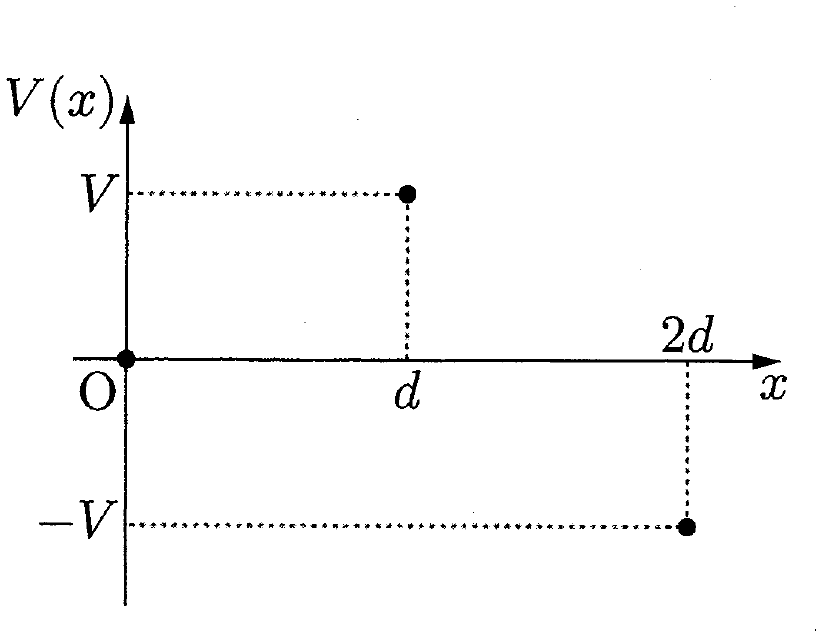
\includegraphics[keepaspectratio,width=58mm]{fig/n24_a42_zu1.png}\end{center}
       極板間には一様な電場が作られているので，電位の変化は各極板間で一定になっている．よって$V(x)$のグラフは各極板間で直線になるので，$V(x)$のグラフは次図のようになる．
       \begin{center}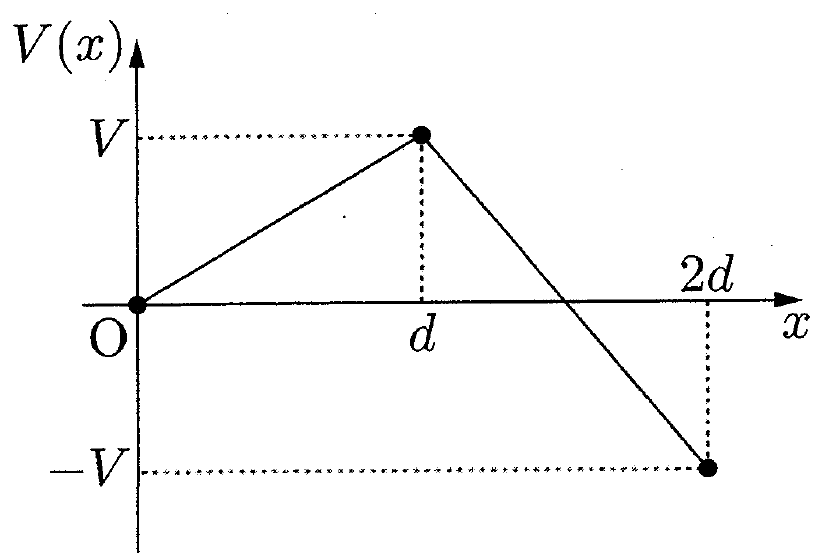
\includegraphics[keepaspectratio,width=58mm]{fig/n24_a42_zu2.png}\end{center}
       また，このグラフを数式化すると，$V(x)\U{V}$は
       \[\left\{\begin{aligned}
        &\frac{V}{d}x&&(0\leqq x\leqq d\U{m})\\
        &3V-\frac{2V}{d}x&&(d\leqq x\leqq 2d\U{m})
       \end{aligned}\right.\]
       \hspace*{\fill}\Ans
\end{komon}

\MonN[\Sitei]{43}{点電荷による電場と電位}\par\nopagebreak
\begin{sisin}
点電荷の作る電場と電位の式の適用に注意．まず，電場の強さの$E=k\dfrac{|Q|}{r^2}\U{N/C}$は大きさのみを求める式（電気量$Q$は絶対値を取って代入する）であり，向きについては別途考える必要があるが，{\gtfamily 電荷の右と左で向きが逆になる}ことに注意せよ．一方，点電荷による電位の式$V=k\dfrac{Q}{r}\U{V}$の方は向きを考える必要はない（電気量$Q$は絶対値を取らずにそのまま代入する）が，点電荷からの距離$r\U{m}$の表式が電荷の右側と左側とで異なることに注意せよ．

なお，多数の電荷がある場合はその重ね合わせとして電場や電位を求めることができる．電場（ベクトル量）については向きを考えた上で重ね合せる必要があるが，電位（スカラー量）については向きを考える必要はなく，単純和を取ればよい．
\end{sisin}
\KaiHead
\begin{komon}
\ko{1} $x$軸正の向きを電場の正の向きとする．まず原点にある$+2q$の点電荷について考えると，これが座標$x\U{m}$の位置に作る電場の強さは，原点から$x\U{m}$までの距離が$|x-0|\U{m}$であることに注意して，
       \[k\frac{2q}{|x-0|^2}=\frac{2kq}{x^2}\]
       であり，点電荷から遠ざかる向きに電場が作られる．よって，原点の電荷$+2q$が作る電場は，向きを符号で表すと，
       \[E_{\mathrm{O}}(x)=\left\{\begin{aligned}
         &+\frac{2kq}{x^2}\U{N/C}&&(x>0)\\
         &-\frac{2kq}{x^2}\U{N/C}&&(x<0)
       \end{aligned}\right.\]
       である．

       次に，$\mathrm{A}$点にある$-q$の点電荷について考えると，これが座標$x\U{m}$の位置に作る電場の強さは，$\mathrm{A}$点から$x\U{m}$までの距離が$|x-d|\U{m}$であることに注意して，
       \[k\frac{q}{|x-d|^2}=\frac{kq}{(x-d)^2}\]
       であり，点電荷に近づいてくる向きに電場が作られる．よって，$\mathrm{A}$点の電荷$-q$が作る電場は，向きを符号で表すと，
       \[E_{\mathrm{A}}(x)=\left\{\begin{aligned}
         &-\frac{kq}{(x-d)^2}\U{N/C}&&(x>d)\\
         &+\frac{kq}{(x-d)^2}\U{N/C}&&(x<d)
       \end{aligned}\right.\]
       である．電場を合成するには，向きを考慮して合成すればよく，
       \[E(x)=E_{\mathrm{O}}(x)+E_{\mathrm{A}}(x)\]
       である（注：向きは符号で表しているのでこの式で向きを考慮して合成したことになる）．よって，$E(x)\U{N/C}$は
       \[\left\{\begin{aligned}
         &\frac{2kq}{x^2}-\frac{kq}{(x-d)^2}&&(d<x)\\
         &\frac{2kq}{x^2}+\frac{kq}{(x-d)^2}&&(0<x<d)\\
         &-\frac{2kq}{x^2}+\frac{kq}{(x-d)^2}&&(x<0)
       \end{aligned}\right.\]
       \hspace*{\fill}\Ans
\ko{2} まず原点にある$+2q$の点電荷について考えると，原点から$x\U{m}$までの距離が$|x-0|\U{m}$であることに注意して，この点電荷は座標$x\U{m}$の位置に
       \[V_{\mathrm{O}}(x)=k\frac{+2q}{|x-0|}=k\frac{2q}{|x|}\U{V}\]
       の電位を作る．

       次に，$\mathrm{A}$点にある$-q$の点電荷について考えると，原点から$x\U{m}$までの距離が$|x-d|\U{m}$であることに注意して，この点電荷は座標$x\U{m}$の位置に
       \[V_{\mathrm{A}}(x)=k\frac{-q}{|x-d|}\U{V}\]
       の電位を作る．電位については単純和を取って重ね合わせればよいので，
       \[V(x)=V_{\mathrm{O}}(x)+V_{\mathrm{A}}(x)\]
       以上より，
       \[V(x)=\frac{2kq}{|x|}-\frac{kq}{|x-d|}\U{V}\]
       であり，絶対値を外すと，$V(x)\U{V}$は
       \[\left\{\begin{aligned}
         &\frac{2kq}{x}-\frac{kq}{x-d}&&(x>d)\\
         &\frac{2kq}{x}-\frac{kq}{d-x}&&(0<x<d)\\
         &\frac{2kq}{-x}-\frac{kq}{d-x}&&(x<0)
       \end{aligned}\right.\]
       \hspace*{\fill}\Ans
\end{komon}
\begin{bsHosoku}{参考}
(1)は先に(2)を求めてから電位と電場の関係式に従って求めてもよい．電位と電場の関係式は
\[E(x)=-\frac{dV}{dx}\]
であるから，(2)の各式を微分すれば(1)の答えが得られる．例えば$x>d$について示すと，
\[\begin{aligned}
 E(x)&=-\frac{d}{dx}\left(\frac{2kq}{x}-\frac{kq}{x-d}\right)\\
     &=\frac{2kq}{x^2}-\frac{kq}{(x-d)^2}
\end{aligned}\]
となり，確かに(1)で求めた答えに一致する．
\end{bsHosoku}

\Rank{C問題}
\MonN{44}{クーロンの法則と力のつり合い}\par\nopagebreak
\begin{sisin}
$\mathrm{P}$に作用するクーロン力をひとつずつ考えようとすると大変なことになる．しかし，B問題［37］などで見たように，{\gtfamily 同じ大きさを持つ二つの電荷が及ぼす力（もしくは電場）を合成すると，ちょうど一つの軸に沿った力（もしくは電場）になる}ことを利用すると，比較的簡単に$\mathrm{P}$に作用するクーロン力の和を求めることができる．どの電荷とどの電荷を組み合わせるのが簡単なのかをよく考えながら問題に取り組んでいこう．
\end{sisin}
\KaiHead
まず，$\mathrm{O}$点に質点$\mathrm{P}$を置いた場合について考える．8個の電荷を，$(x,\ y)$座標の等しい二つずつの電荷4組に分けて，それぞれの組が$\mathrm{P}$にどれだけの力を及ぼすのかを考える．

まず，座標$(+a,\ +a,\ \pm a)$の二つの電荷のペアに着目し，この二つの電荷が$\mathrm{P}$に作用するクーロン力の和を求める．
\begin{center}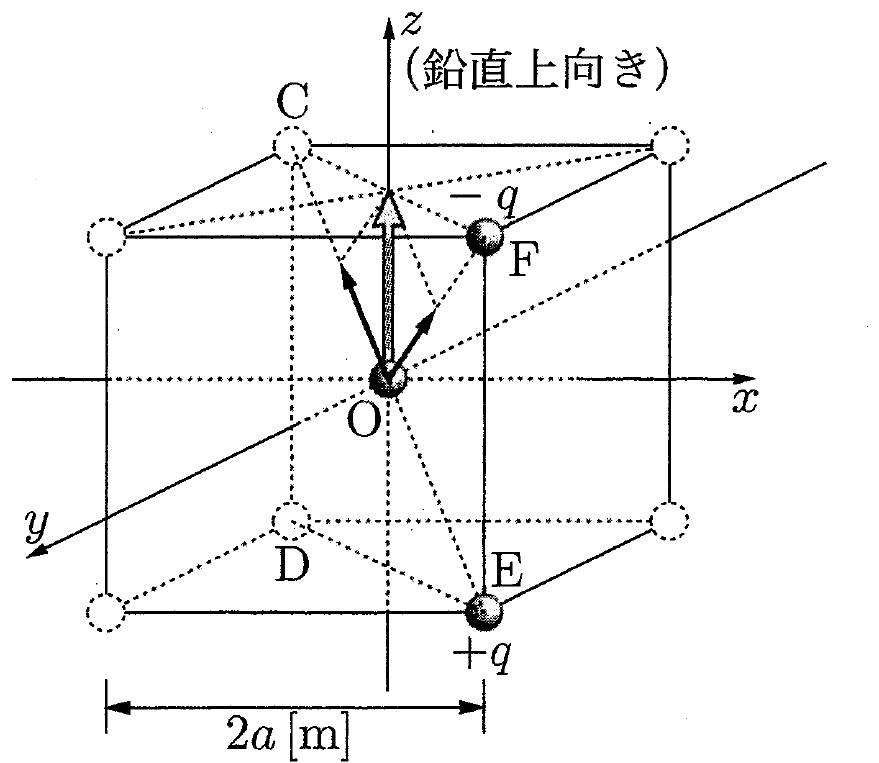
\includegraphics[keepaspectratio,width=62mm]{fig/n24_a44_zu1.png}\end{center}
前図の$\mathrm{CDEF}$断面に着目すると，
\[\overline{\mathrm{OF}}=\overline{\mathrm{OE}}=\sqrt{3}\,a\U{m}\]
であり，$\mathrm{O}$点に置かれた正電荷に対しては，$\mathrm{E}$の正電荷は斥力を作用するので$\overrightarrow{\mathrm{EO}}$向きに，また$\mathrm{F}$の負電荷は引力を作用するので$\overrightarrow{\mathrm{OF}}$向きに力を作用する．その大きさは，いずれも
\[f=k\frac{qQ}{\left(\sqrt{3}\,a\right)^2}\U{N}\]
である．$\mathrm{CDEF}$断面での力の作用図を書き出すと次図のようになる．
\begin{center}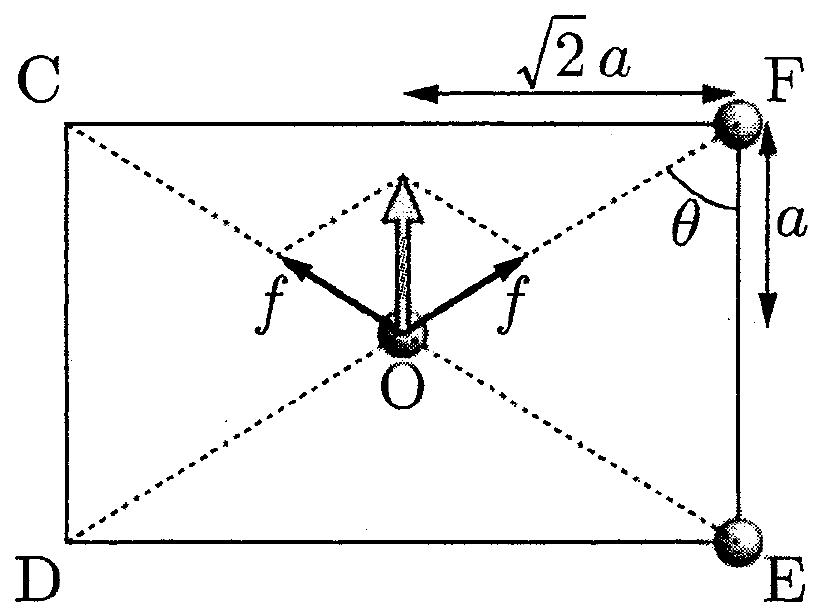
\includegraphics[keepaspectratio,width=58mm]{fig/n24_a44_zu2.png}\end{center}
よって，$\angle\mathrm{OFE}=\theta$とおき，この二つのクーロン力のベクトル合成を取ると，$\cos\theta=\dfrac{1}{\sqrt{3}}$であるから
\[f\times 2\cos\theta=\frac{2kqQ}{3\sqrt{3}\,a^2}\U{N}\]
となる．

これと全く同様の議論が，$(+a,\ -a,\ \pm a)$のペア，$(-a,\ +a,\ \pm a)$のペア，$(-a,\ -a,\ \pm a)$のペアについても出来るので，中心に置いた質点$\mathrm{P}$の受けるクーロン力は上向きに，
\[4\times\frac{2kqQ}{3\sqrt{3}\,a^2}=\frac{8kqQ}{3\sqrt{3}\,a^2}\U{N}\]
となり，これが重力とつり合うのだから，重力加速度の大きさを$g\U{m/s^2}$とすると，力のつり合いより
\[\frac{8kqQ}{3\sqrt{3}\,a^2}=mg\]
が成立する．

次に，$\mathrm{A}$点にこの質点$\mathrm{P}$を配置した場合について考える．まず，上面の四つの$-q\U{C}$が$\mathrm{A}$点に置いた$\mathrm{P}$に作用するクーロン力について考えると，いずれも大きさが
\[k\frac{qQ}{\left(\sqrt{2}\,a\right)^2}\U{N}\]
の引力であり，向きは次図に示す通りであるから，これらは互いに打ち消し合う．
\begin{center}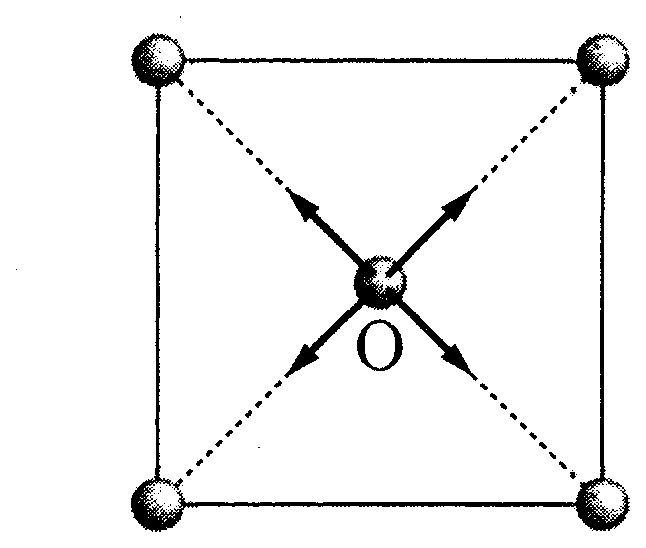
\includegraphics[keepaspectratio,width=48mm]{fig/n24_a44_zu3.png}\end{center}
次に下面の四つの$+q\U{C}$が$\mathrm{A}$点に置いた$\mathrm{P}$に作用するクーロン力について考える．これらの$+q\U{C}$と$\mathrm{A}$点との距離は
\[\sqrt{(2a)^2+\left(\sqrt{2}\,a\right)^2}=\sqrt{6}\,a\U{m}\]
であるから，各々の電荷は大きさが
\[f_1=k\frac{qQ}{\left(\sqrt{6}\,a\right)^2}\U{N}\]
の斥力を及ぼす．
\begin{center}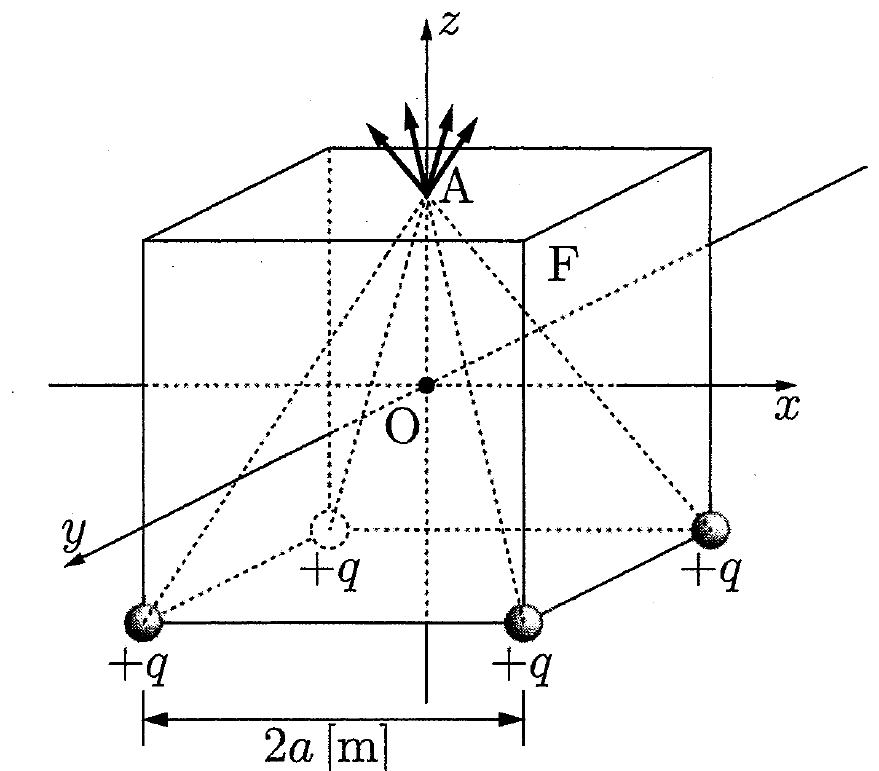
\includegraphics[keepaspectratio,width=62mm]{fig/n24_a44_zu4.png}\end{center}
これらのベクトル合成を取るにあたって，先ほどの$\mathrm{CDEF}$断面に着目すると，
\begin{center}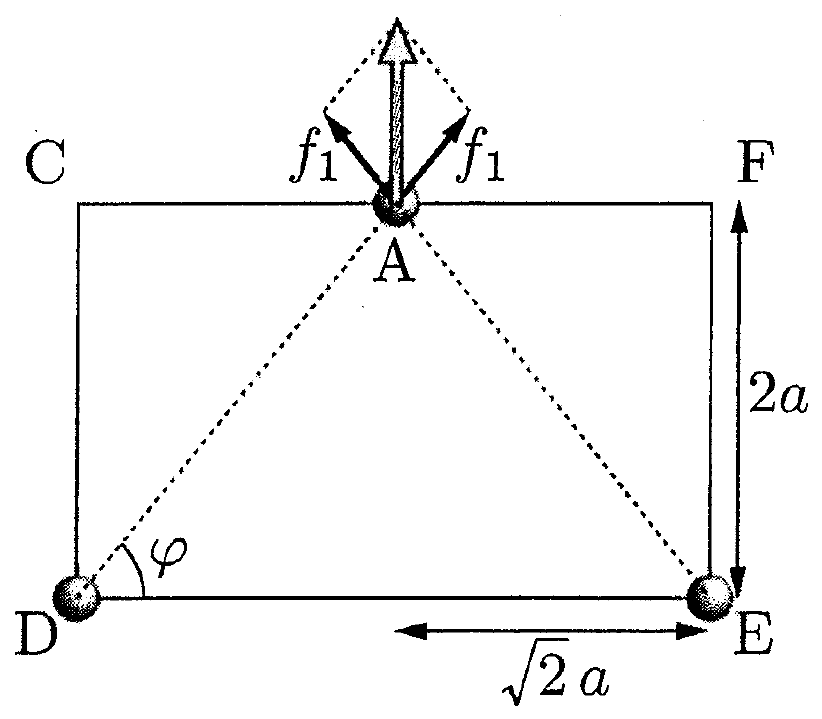
\includegraphics[keepaspectratio,width=58mm]{fig/n24_a44_zu5.png}\end{center}
前図の$\angle\mathrm{ADE}=\varphi$とおくと$\sin\varphi=\dfrac{2}{\sqrt{6}}$であるから，この二つの力の合力は，
\[f_1\times 2\sin\varphi=\frac{2kqQ}{3\sqrt{6}\,a^2}\U{N}\]
である．同様の議論が$(+a,\ -a,\ -a)$と$(-a,\ +a,\ -a)$の電荷のペアについても言えるので，下面四つの正電荷による合力は，$+z$向きに大きさ
\[\frac{2kqQ}{3\sqrt{6}\,a^2}\times 2=\frac{4kqQ}{3\sqrt{6}\,a^2}\U{N}\]
となる．質点$\mathrm{P}$にはこのクーロン力と，下向きの重力$mg\U{N}$の二つが作用する．ここで，この二つの力の大小関係を比較すると，
\[\frac{\dfrac{4kqQ}{3\sqrt{6}\,a^2}}{mg}=\frac{\dfrac{4kqQ}{3\sqrt{6}\,a^2}}{\dfrac{8kqQ}{3\sqrt{3}\,a^2}}=\frac{1}{2\sqrt{2}}\]
となるので重力の方が大きい．以上より，二つの合力は下向きである．またその大きさは，
\[\begin{aligned}
 mg-\frac{4kqQ}{3\sqrt{6}\,a^2}&=mg-\frac{mg}{2\sqrt{2}}\\
 &=\left(1-\frac{\sqrt{2}}{4}\right)mg\U{N}
\end{aligned}\]
であるから，{\gtfamily 向きは鉛直下向き}で，大きさは重力の$1-\dfrac{\sqrt{2}}{4}$倍である．\Ans

\MonN{45}{等電位線と仕事}\par\nopagebreak
\begin{sisin}
電荷が移動して電位が変化すると，電荷の持つ位置エネルギー$U=q\cdot V\U{J}$が変化する．よって，電荷を動かすためには位置エネルギーの増加分に相当するだけの仕事を与えてやる必要がある．

電場と電位は一直線上の場合には$E=-\dfrac{dV}{dx}$の関係式で結ばれているが，本問のような平面上，もしくは空間中の場合には，電場の向きは，{\gtfamily 等電位線を等高線とみなした場合の最大傾斜角方向}になり，その傾斜の傾きが電場の強さになる．よって，等電位線の間隔が狭いところでは電位の傾きが大きく，したがって電場の強さが大きいと判断できる．
\end{sisin}
\KaiHead
\begin{komon}
\ko{1} 電荷を移動させると，電荷の存在する位置の電位が変わっていくため，電荷の持つ位置エネルギーが変化する．よって，電荷を動かすためにはこの位置エネルギーの変化分だけの仕事を外力によって与えてやる必要がある．例えば$\mathrm{A}$, $\mathrm{B}$点における電位はそれぞれ$20$, $20\U{V}$であるから，区間$\mathrm{AB}$で外力がした仕事$W_{\mathrm{AB}}\U{J}$は，移動後の位置エネルギーから移動前の位置エネルギーを差し引けば求められる．点$\mathrm{X}$の電位を$V_X\U{V}$と表すことにすると，
       \[\begin{aligned}
        W_{\mathrm{AB}}&=(+5)\cdot V_{\mathrm{B}}-(+5)\cdot V_{\mathrm{A}}\\
        &=(+5)(20-20)=0\U{J}\Ans
       \end{aligned}\]
       同様にして，
       \[\begin{aligned}
        W_{\mathrm{BC}}&=(+5)\cdot V_{\mathrm{C}}-(+5)\cdot V_{\mathrm{B}}\\
        &=(+5)(10-20)=-50\U{J}\Ans\\
        W_{\mathrm{CD}}&=(+5)\cdot V_{\mathrm{D}}-(+5)\cdot V_{\mathrm{C}}\\
        &=(+5)(40-10)=150\U{J}\Ans\\
        W_{\mathrm{DE}}&=(+5)\cdot V_{\mathrm{E}}-(+5)\cdot V_{\mathrm{D}}\\
        &=(+5)(20-40)=-100\U{J}\Ans\\
        W_{\mathrm{EA}}&=(+5)\cdot V_{\mathrm{A}}-(+5)\cdot V_{\mathrm{E}}\\
        &=(+5)(20-20)=0\U{J}\Ans
       \end{aligned}\]
\ko{2} (1)の結果より，
       \[\begin{aligned}
        W&=W_{\mathrm{AB}}+W_{\mathrm{BC}}+W_{\mathrm{CD}}\\
         &\qquad{}+W_{\mathrm{DE}}+W_{\mathrm{EA}}\\
         &=0+(-50)+150+(-100)+0\\
         &=0\U{J}\Ans
       \end{aligned}\]
       \begin{bekkai}
       (1)の仕事の総和とは，$\mathrm{A}$点から移動を始めて，最終的に再び$\mathrm{A}$点に戻すときの仕事である．結局再び$\mathrm{A}$点に戻ったので，全体での位置エネルギー変化は$0$である．よって，必要な仕事は
       \[W=0\U{J}\]
       となる．
       \end{bekkai}
       \begin{chuu}
       一見すると物体を動かすのには仕事が必要だからこの結果はおかしいように思えるかもしれない．これは，ある区間では外力が荷電粒子に仕事をするが，ある区間では逆に外力の方が荷電粒子から仕事をなされ，その総和が$0$になることを意味している．
       \end{chuu}
\ko{3} 等電位線の幅が狭いほど電位の傾きが大きく電場が強いので，図から，$\mathrm{D}$点の方が$\mathrm{A}$点よりも電場が強い．\Ans
       \begin{chuu}
       $\mathrm{D}$点の方が$\mathrm{A}$点よりも電位が高い（$40\U{V}$，$20\U{V}$ゆえ）が，この{\gtfamily 電位そのものの大小関係と電場の大小関係とは無関係}であることに注意．電場は電位の傾きであり，電位そのものの大きさではないからである（高さと傾きに直して考えれば分かりやすい．海抜が高いところにあるなだらかな斜面と，海抜が低いところにある急な斜面とを比べた場合，海抜の高さは前者の方が高いが，坂道の傾斜は後者の方が大きい．このように，高さの大小関係と傾きの大小関係とは無関係である）．
       \end{chuu}
\end{komon}

\MonN{46}{電場と仕事}\par\nopagebreak
\begin{sisin}
点電荷による電場と一様電場との合成の問題であるが，このような場合に，まず先に各々の電気力線を合成して空間中に出来る電場の全体像を把握する，という考え方で攻めるのは難しい（考えてみよ）．そこで，敢えて電場や電位は合成せず，点電荷によるもの，一様電場によるものをひとつずつ考えて，あとからその二つの和を取って合成する，という手法で攻めよう．
\end{sisin}
\KaiHead
\begin{komon}
\ko{1} まず，点アに負電荷$-q\U{C}$を置くと，これは$\mathrm{O}$点にある正電荷$+q\U{C}$から右向きの引力を受ける．よって，この負電荷$-q\U{C}$がこのまま静止を続けるためには，一様な電場から，左向きに同じ大きさの力を受けなければならない．一様電場から{\gtfamily 負電荷が左向きに力を受ける}ためには，右向きに電場がかかっている必要がある．よって，一様な電場の向きは右向き（点ア$\rightarrow$点オの向き）である．\Ans

       点$\mathrm{O}$にある正電荷からこの負電荷が受ける引力は右向きで，その大きさは，
       \[k\frac{|(-q)\cdot(+q)|}{r^2}=\frac{kq^2}{r^2}\U{N}\]
       である．右向きの一様電場の強さを$E\U{V/m}$と置くと，この負電荷$-q\U{C}$は一様電場から左向きに大きさ$|(-q)\cdot E|\U{N}$の力を受けており，これが上述の力とつり合っているので，力のつり合いの式は，
       \[\frac{kq^2}{r^2}=qE\]
       である．これを解いて，
       \[E=\frac{kq}{r^2}\U{V/m}\Ans\]
\ko{2} 小球$\mathrm{M}$をア$\rightarrow$イ$\rightarrow$ウ$\rightarrow$エと移動させる際に外力が小球$\mathrm{M}$に対してなした仕事は，小球の位置エネルギー変化に利用されるので，小球$\mathrm{M}$の位置エネルギー変化を求めればよい．

       この空間に作られている電位は，一様電場によるものと点電荷によるものとの合成（単純和，スカラー合成）であるから，点アと点エの電位の差を求める際には，一様電場が作る電位の差と，点電荷が作る電位の差とをそれぞれ個別に求めて，これを足し合わせれば求められる．

       まず，一様電場のみに着目する．電気力線は次図のようになっており，電気力線と等電位線とが直交することに注意すると，点エの電位は点ケの電位と同一である．
       \begin{center}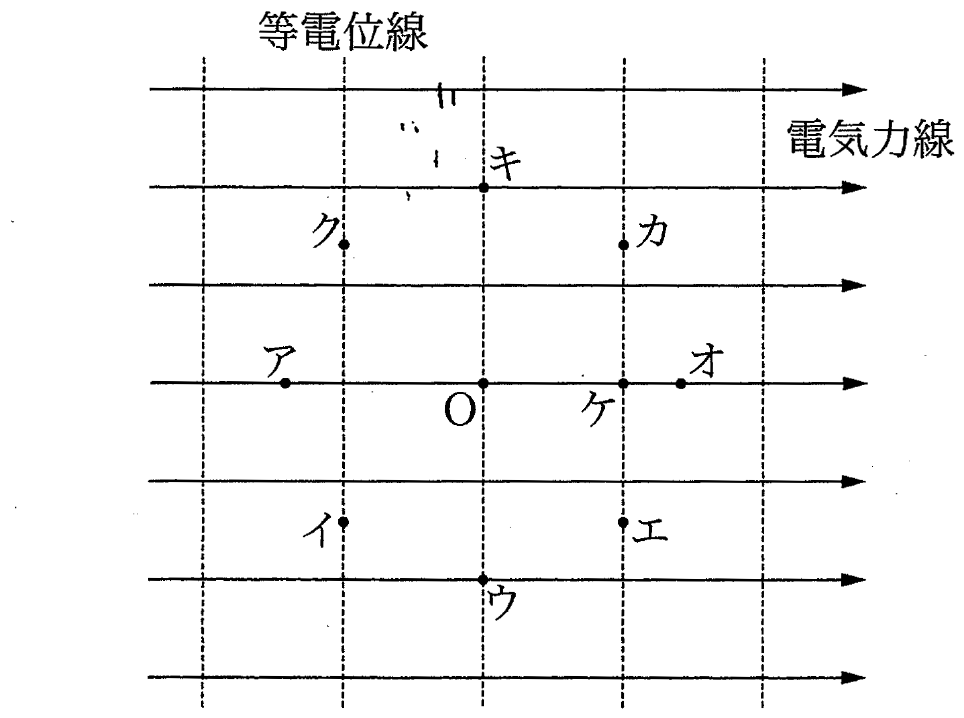
\includegraphics[keepaspectratio,width=68mm]{fig/n24_a46_zu1.png}\end{center}
       点アと点ケの距離は$\left(\dfrac{\sqrt{2}}{2}+1\right)r\U{m}$であるから，点アと点ケの電位の差，すなわち点アと点エの電位の差は
       \[E\times\left(\frac{\sqrt{2}}{2}+1\right)r=\left(\frac{\sqrt{2}}{2}+1\right)\frac{kq}{r}\U{V}\]
       であり，また電気力線の向きから判断して，点アの方が高電位である．

       一方，点電荷のみに着目すると，電気力線および等電位線は次図のようになるので，点エの電位は点アの電位と同一になる．
       \begin{center}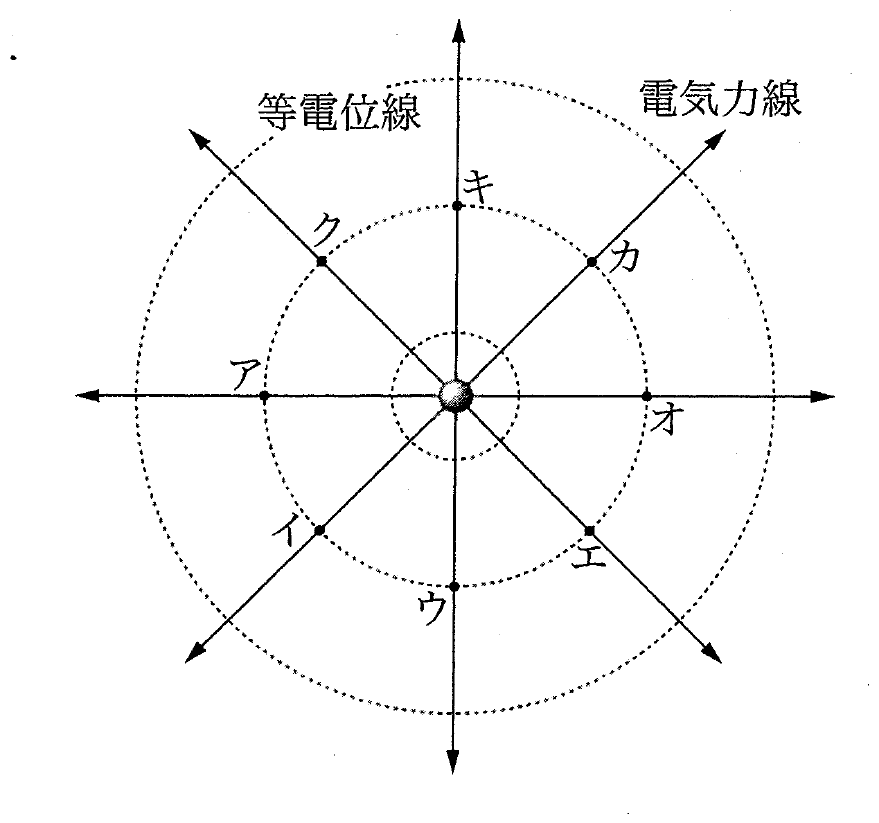
\includegraphics[keepaspectratio,width=62mm]{fig/n24_a46_zu2.png}\end{center}
       よって，この図より明らかに，点アと点エの電位の差は$0\U{V}$である．

       以上より，点アに対する点エの電位は，この二つの和を取って，
       \[\begin{aligned}
        \Delta V&=-\left\{\left(\frac{\sqrt{2}}{2}+1\right)\frac{kq}{r}\right\}+0\\
        &=-\left(\frac{\sqrt{2}}{2}+1\right)\frac{kq}{r}\U{V}
       \end{aligned}\]
       であり，この小球$\mathrm{M}$を移動させた場合の位置エネルギー変化は
       \[\Delta U=(-q)\cdot\Delta V=\left(\frac{\sqrt{2}}{2}+1\right)\frac{kq^2}{r}\U{J}\]
       である．よって，外力が$\mathrm{M}$に対してした仕事は，
       \[W=\Delta U=\left(\frac{\sqrt{2}}{2}+1\right)\frac{kq^2}{r}\U{J}\Ans\]
\end{komon}

\end{multicols}
